\documentclass[a4paper,12pt,twoside,openany]{report}
\usepackage{graphicx}
\usepackage{xspace}
\usepackage{url}

% font and encoding setup
\usepackage[utf8]{inputenc}
\usepackage[T1]{fontenc}
\usepackage{newcent}

% references
\usepackage{prettyref}
\newrefformat{cha}{Chapter~\ref{#1}}
\newrefformat{sec}{Section~\ref{#1}}
\newrefformat{tab}{Table~\ref{#1}}
\newrefformat{fig}{Figure~\ref{#1}}

% page setup
\usepackage[margin=1.5in]{geometry}
% put section numbers in the margin
\makeatletter
\def\@seccntformat#1{\protect\makebox[0pt][r]{\small\csname the#1\endcsname\quad}}
\makeatother
\usepackage{fancyhdr}
\usepackage{setspace}
\raggedbottom
\renewcommand\footnoterule{\vfill\hrule\vspace{6pt}}

% set up floats
\usepackage[font=small,labelfont=bf]{caption}
\renewcommand{\topfraction}{.8}
\renewcommand{\bottomfraction}{.8}
\renewcommand{\textfraction}{.2}
\renewcommand{\floatpagefraction}{.8}
\newcommand{\figwidth}{.8\textwidth}

\newcommand{\note}[1]{\marginpar{\begin{tiny}#1\end{tiny}}}
%\suppressnotes

% ignore Overfull \vbox messages
\vfuzz 2pt

\clubpenalty=9999
\widowpenalty=9999
\interfootnotelinepenalty=9999

% allow some extra space for paragraph breaking
\setlength{\emergencystretch}{1em}

\newcommand{\thesistitle}{Cluster Storage for Commodity Computation}
\newcommand{\thesistitlebig}{Cluster Storage for\\ Commodity Computation}

% pdf settings
\usepackage[
  %pdftex,
  bookmarks=true,
  linkbordercolor={0 0 1},
  pagebackref=true,
  plainpages=false,
  pdfpagelabels=true,
  hypertexnames=false,
  breaklinks=true]{hyperref}
\hypersetup{
  pdfauthor   = {Russell Glen Ross},
  pdftitle    = {\thesistitle},
  pdfsubject  = {A dissertation submitted to the University of Cambridge
                  for the degree of Doctor of Philosophy},
  pdfkeywords = {File Systems, Distributed Systems, Cluster Storage,
                 Commodity Computation, Virtualization},
  pdfcreator  = {LaTeX with hyperref package},
  pdfproducer = {pdftex}}

\begin{document}

% front matter

\pagestyle{empty}
% title page

\begin{titlepage}
\begin{center}
\vspace*{\fill}

\huge
\thesistitlebig

\vfill
\vfill

\huge
Russell Glen Ross\\[6mm]
\large
Wolfson College

\vfill

\includegraphics[width=70pt]{figures/camshield}
\vfill

\large
A dissertation submitted to the University of Cambridge\\
for the degree of Doctor of Philosophy

\vfill

% December 2006
Draft of \today

\vspace*{\fill}
\end{center}
\end{titlepage}

\cleardoublepage

% set up page headers and footers
\pagestyle{fancyplain}
\renewcommand{\headrulewidth}{0pt}
\renewcommand{\footrulewidth}{0pt}
\renewcommand{\plainheadrulewidth}{0pt}
\renewcommand{\plainfootrulewidth}{0pt}
\renewcommand{\chaptermark}[1]{\markboth{#1}{\thechapter.\ #1}}
\renewcommand{\sectionmark}[1]{\markright{\thesection.\ #1}}
\headheight 15pt

% no headers for the front matter
\lhead{}
\rhead{}
\cfoot{}

% number the front matter in roman numerals
\pagenumbering{roman}
\lfoot[\sl\thepage]{}
\rfoot[]{\sl\thepage}

% preface

\chapter*{Preface}

{
\parskip 10pt

\noindent This dissertation is the result of my own work and includes nothing which is the outcome of work done in collaboration except where specifically indicated in the text.

\noindent This dissertation is not substantially the same as any I have submitted for a degree or diploma or any other qualification at any other university. No part of this dissertation has already been, or is currently being submitted for any such degree, diploma or other qualification.

\noindent This dissertation does not exceed sixty thousand words.
}
\vfill

\noindent This dissertation is copyright \copyright~2006 Russell Glen Ross

\chapter*{Summary}

Standards in the computer industry have made basic components and entire architectures into commodities, and now software and services are following. By an accident of timing, these two trends are interlinked. Commodity hardware is being used increasingly for the heavy lifting formerly reserved for specialized platforms through the advent of GRID computing and clusters of cheap hardware as used by Google and other companies. Improved web interfaces, widespread internet access, and cheap servers make it practical for many software services to be hosted by specialized providers instead of being managed directly by users and corporate IT departments.

Modern updates to virtualization technology make it practical to subdivide these commodity servers and manage groups of heterogeneous services using commodity operating systems and tools. Computation as a commodity is soon to follow, and some progress has already been made in making this a reality.

In this dissertation, I argue for the adoption of \emph{service clusters}---clusters of commodity machines managed by a single administrator, but running services in virtual machines for arbitrary, untrusted clients---as the basic building block for an economy of \emph{flexible commodity computation}. I then outline the requirements such a platform imposes on its storage system and argue that they are necessary for service clusters to be practical, but not found in existing systems.

Next I introduce the \envoy file system, a distributed file system for service clusters. In addition to meeting the needs of service clusters, \envoy introduces a novel file distribution scheme that organizes metadata management according to runtime usage patterns; in effect, the file system is partitioned to give control of each part to the client that uses it the most, and that client in turn acts as a server with caching for other clients that require concurrent access. This allows it to provide scalability that is limited by only by actual contention, and a perfectly consistent cache distributed across the cluster.
% acknoledgements

\chapter*{Acknowledgements}

Thanks everyone.


% table of contents

\onehalfspace
\parskip 0pt plus 1pt

\renewcommand\contentsname{Table of Contents}
\tableofcontents

% \clearpage
% \addcontentsline{toc}{chapter}{\listtablename}
% \listoftables
% 
% \clearpage
% \addcontentsline{toc}{chapter}{\listfigurename}
% \listoffigures

% start normal page numbering with page one on the right side
\cleardoublepage
\pagenumbering{arabic}

\parskip 10pt

% page headers with chapter and section names
\makeatletter
  \if@twoside
    \lhead[\fancyplain{}{\sffamily\small\textsl{\leftmark}}]{}
    \rhead[]{\fancyplain{}{\sffamily\small\textsl{\rightmark}}}
  \else
    \lhead[]{\fancyplain{}{\sffamily\small\textsl{\rightmark}}}
  \fi
\makeatother

% main text

\chapter{Introduction}

This dissertation presents the design and implementation of a distributed file system. The design is motivated by the requirements of a new environment that emerges at the intersection of two trends: the renaissance of machine virtualization as a tool for hardware management, and the increasing use of commodity hardware and software for problems at the high end of the computation spectrum. 

\section{Motivation}

* Trends: commodity hardware 
* Storage for specific environments
* Storage driven by practical realities
* Competing goals: speed vs reliability, etc.
* POSIX is limited: extend with snapshots, forks, etc.
* VMs

\section{Contributions}

* Argument for commodity computing needing a platform
* Argument for services as basic unit of management
* Argument for clusters of services as platform for commodity computing
* Argument for new storage system to meet needs of this platform
* Design of Envoy file system
* Prototype and evaluation of Envoy

\section{Outline}
\begin{enumerate}
\item Background: commodity computing (GRID, clusters, utility computing), virtual machines, file systems
\item Motivation: state of commodity computing, argument for service-based economy, proposal and definition of service clusters
\item Design: Needs of storage clusters, high-level design of Envoy, management and how it appears to users, storage layer, envoy layer, tricky features and operations
\item Prototype implementation
\item Evaluation
\item Conclusion
\end{enumerate}
\chapter{Background}

\section{Commodity computing}


Similar idea as network appliances: \cite{sapuntzakis03}. SoftUDC: software-based data center \cite{kallahalla}. Utilification \cite{wilkes04}.

\subsection{Network of workstations}
Networks of workstations (NOW)\cite{anderson95a}

\subsection{Clusters}

Embarassingly parallel problems

CARD for cluster monitoring\cite{anderson97}

Fast crash recovery verses redundancy\cite{baker94}

Partition cloning \cite{rauch}

TranSend was written for and the Inktomi search engine adapted to a layered cluster platform for scalable, homogeneous network services. Services composed of a few distinct types of actors could be managed by a common platform that provided monitoring and allocation of the component parts over the cluster. This type of platform exemplifies many of the advantages of clusters for network services, including load balancing, incremental scaling, fault tolerance, and high availability, but the implementation was limited to ``embarassingly parallel'' problems with trusted components and a custom state management system backed by a commercial SAN \cite{fox}. The authors were able to demonstrate that scalability was limited more by bandwidth into the cluster than by communication within it or coordination overhead.

\subsection{GRID}
\cite{zhao04}

\subsection{Utility computing}
\subsection{Hosted services}

\section{Virtualization}

\subsection{Virtual machine monitors}
IBM System/370 \cite{gum}
Disco
Denali
Xen \cite{barham}
Live migration \cite{clark} \cite{sapuntzakis02}
Terra \cite{garfinkel}
VMWare
vMatrix \cite{awadallah}
IBM Managed Hosting

\subsection{XenoServers}
\cite{kotsovinos04a,kotsovinos04b}

Ventana \cite{pfaff}

\section{Storage systems}

Storage is a fundamental component of all general-purpose computer systems. A combination of high storage density, random access, and low cost have made magnetic storage on rotating platters the dominant medium for durable storage. The time to access a random byte of data from a disk is typically measured in milliseconds, while for DRAM this time drops roughly six orders of magnitude to a nanosecond scale, and that gap is continuing to grow.

Because disks are so slow, storage systems are designed around the goal of accessing the disk as little as possible, and favoring sequential access to avoid costly seek delays. Effective use of cache is vital to this goal, and specialized storage systems tuned to specific system architectures and expected workloads are worthwhile because of the potential speed gains over more general systems.

Storage systems have been studied extensively, and one purpose of this section is to survey related work that has influenced this dissertation. A second purpose relates to the thesis of this work, which argues that a new environment justifies a new storage architecture. The works discussed here are presented in the context of the environments that inspired them, in part to establish a pattern of symbiosis between storage architectures and computation environments, a pattern at the heart of the present work. Envoy, the file system introduced in this dissertation, is discussed briefly in this section to relate it to prior work, but details of its design are reserved for later chapters.

\subsection{Local file systems}

Disks are mechanical devices and their performance is limited primarily by the need to physically position the disk head over the correct part of the platter to access data. File systems designed for local disks achieve performance by minimizing the physical movement required. Disk access can be reduced through caching, and hardware latency can be minimized by arranging data on the disk to minimize movement. Correctness and reliability tend to trump performance as design considerations, however, and the wide variety of possible workloads makes it difficult to pick clear winners from competing designs.

The Berkeley Fast File System (FFS) was the first to optimize data layout for performance by clustering related information. Block metadata is distributed across the disk to be near the file data it describes, file metadata is grouped for files in the same directory, and blocks in the same file are grouped whenever possible \cite{mckusick}. \emph{Clustering}, as this design is called, exploits concepts that extend beyond local file systems: the same expectations of correlated access can be exploited to reduce latency when accessing data across the network.

File system tracing reveals how files are accessed in real systems \cite{ousterhout}. Most files accessed are small, but size distributions are skewed enough that most data transferred is from large files. Writes are less common than reads, and most files are short-lived. Files access is typically sequential, and most files are read from or written to in their entirety. These trends have proved resiliant over time, though the scale has increased and largest files in typical systems have grown much larger \cite{ruemmler,gibson98b}.

As cache sizes grow, more requests can be satisfied without consulting the disk, and designs can assume that many read requests can be served from memory. All writes whose effects are not quickly undone have to go to disk eventually, so despite being fewer overall, writes requests can dominate the mix of operations that penetrates the cache and reaches the disk. Furthermore, updates often involve metadata changes as well, potentially requiring multiple costly disk seeks even for small updates.

The log-structured file system (LFS) addressed this problem by borrowing from database design and making the entire file system an append-only log. Writes are gathered and written as sequential chunks on disk, with relevant metadata rewritten instead of updating existing structures directly \cite{rosenblum}. \emph{Journaling} file systems apply the same idea to other file system types, logging only the intent to update metadata. Once the log is committed, the conventional structures can be updated asynchronously while still guaranteeing durability in the face of a system crash \cite{hagmann,sweeney,tweedie}. Breaking the chain of required metadata commits is also the objective of \emph{soft updates}, a technique that involves careful rearrangement of data in the buffer cache to permit delays and reordered writes \cite{ganger94}.

Studies comparing FFS with LFS \cite{seltzer95} and journaling with soft updates \cite{seltzer00} reveal a complicated picture. The requirement of cleaner process in LFS to reclaim space from the log interferes under some workloads, and updates to clustered file systems reduce the ordered-write problem enough to keep it competitive with small file updates. Will all of these systems, it is careful attention to the motion of the disk head that leads to good performance.

% TODO: This is a really weak section
What's the point?  How does this apply to Envoy?

In distributed systems or even local RAID arrays \cite{patterson}, higher-order effects can further distort the picture \cite{stein05}.

\subsection{Client-server file systems}

If local file systems can be characterized by how they manage disk head motion, distributed file systems are dominated by concerns of data placement and cache management. For a single host, cache management is easy. The OS has a monopoly on the disk and can reconcile any concurrent requests directly. Complications are mainly concerned with deciding when to commit writes to disk to ensure durability in the face of a system crash. Distributed systems must also consider consistency between caches on multiple machines. If a cache delivers an out-of-date version of a file, the application may be led to produce incorrect results.

The Sun Network File System (NFS) was the first widely-used file system for sharing files across hosts \cite{sandberg}. NFS serves many clients from a single server, which hosts the persistent and canonical version of a file. Cache policy is unspecified, with no explicit support from the server. Clients generally cache reads and writes in memory and check with the server before relying on old cache entries (typically in the range of 10s of seconds). Thus an update made by one client is only detected by another when the first has sent the update to the server and the second has checked for an update. Clients can send a constant stream of \texttt{stat} requests to check for updates, but they cannot hasten a delayed update from another client, so they can never be assured of having the latest version of a file. An update to the protocol helped reduce traffic somewhat by performing implicit \texttt{stat} requests and including the results with common operations \cite{pawlowski,callaghan}, but the fundamental problem remained as clients still delay writes to the server. The latest update, NFSv4, includes features to improve cache management by \emph{delegating} complete control of individual files to clients and \emph{revoking} the delegation when other clients seek concurrent access.

Other client-server systems addressed the problem in different ways. The Andrew File System (AFS) \cite{satyanarayanan85,howard} uses the client's disk as a persistent cache with close-to-open semantics. In this scheme, the cache is validated at file open time, and changes forwarded to the server at file close time. To reduce validity checks at file open time, a client can be given a \emph{callback}, meaning that it can assume the file is current unless explicitly notified by the server. These changes improved scalability by enlarging the effective cache size on clients and reducing the load on the server, but they still left open the possibility of conflicting updates by multiple clients. Coda extended AFS to explore the problem of conflict resolution, opening up access to mobile users and allowing clients to continue operating when disconnected from the network \cite{satyanarayanan90,mummert}. DEcorum went the other way, extending AFS to strengthen cache consistency using tokens, as well as interopperate better with existing file systems and reduce recovery time after a crash \cite{kazar}.

The Sprite team observed that---despite the popularity of such systems---most applications do not explicitly account for inconsistencies introduced by the file system, so loosening consistency guarantees in favor of performance gains is a dangerous tradeoff. They sacrificed some performance for full cache consistency by disabling caching for files under contention \cite{baker91,nelson,welch}. Since concurrent access is relatively rare \cite{kistler}, this did not pose a significant problem for overall performance.

In all distributed file systems that permit sharing, there must either be a canonical version of the file (or block \cite{mcgregor}) or some way to reconcile conflicting updates \cite{kistler}. In the former case, some participant is usually nominated as the owner of a particular file through a lease \cite{gray89}, token passing \cite{burrows,mann,kazar}, or some other scheme. Any other host wanting access to the latest version must coordinate through the owner. Ownership may go to the host that provides storage, the one actively using the file, or a third manager host that connects the two \cite{blaze,keleher}. In Envoy, ownership goes to an active user, which then acts as a synchronous server to other users. Unlike Sprite, the principle user can continue to cache the file locally and share its cache with other concurrent users.

Another possibility is to disallow write sharing. The Cedar file system \cite{schroeder} makes all shared files immutable, and turns the problem into one of versioning \cite{gifford}. Venti takes this a step further by storing all file versions permanently and addressing them by a hash of their contents \cite{quinlan}. Since files are never changed or deleted, the store collects a complete history of all historical states of the file system. In workstation environments, it is possible for storage capacity to grow faster than storage is consumed, making this a feasible system, or past versions can be selectively removed as in the local file system Elephant \cite{santry}.

A less drastic approach is to permit snapshots \cite{hitz}, then mark historic versions as read-only with no requirement for cache coordination \cite{warfield}. Envoy employs this dichotomy between active and read-only file versions, implementing cache management only for mutable objects. It does not coalesce identical read-only objects like Venti or Farsite \cite{douceur02}. It could be extended to do so using a lazy, asynchronous process, but it reduces the need by promoting file system forking with copy-on-write as a management tool to avoid creating many of the duplicates in the first place.

Where snapshot systems typically use copy-on-write to transparently combine old data with new, some systems allow explicit stacking of file systems. Spring \cite{khalidi} allows file systems to be layered with optionally synchronized updates as a mechanism for extending functionality by layering in new features. Plan~9 \cite{pike90} allows any file system mount to be layered over another and their contents combined to give each user a custom view of local and remote file systems \cite{pike92}. The copy-on-write NFS server I developed for the XenoServers project \cite{kotsovinos04b} allowes layering instructions to be put in files, where the server immediately notices them and reconfigures the user's view of the file system. These systems can be used as a way to fork a file system, by sharing the common base image and capturing changes in a private layer. Over time this can lead to complex hierarchies of layers, and such systems rely on the semantics of their backing file systems. Envoy can be used in conjunction with a stacking layer, but it already provides explicit support for snapshots and file system forks.

\subsection{Serverless file systems}

While creative caching can alleviate the problem somewhat, all client-server architectures have inherent scaling problems. As a single point of contact for all clients, a server's load grows in proportion to the number of clients, and it also represents a single point of failure. In addition, the duties of a server tend to make it unsuitable for other uses, so such an architecture calls for a dedicated server. As workstations have grown in power, harnessing their excess capacity to cooperate on large problems has become increasingly attractive \cite{anderson95a}.

In xFS, the traditional roles of a server are split and distributed to the clients to yield a serverless architecture \cite{anderson95b}. Hosts can act as clients, managers that coordinate data placement, and/or storage servers that provide disk space, similar to the file system of the earlier LOCUS distributed operating system \cite{walker}. Cache coherency is achieved through an explicit consistency protocol where conflicting client requests are detected and managed.

In addition, the xFS team observed that modern networks make retrieval from a peer's cache faster than from a disk \cite{dahlin94b}, so sharing and coordinating cache across hosts can yield benefits over discrete local caches \cite{dahlin94a}. The resulting protocol was so complex that the team had to employ a formal protocol verifier to get a working implementation \cite{wang98}. While a valid way to manage complexity, reducing complexity through design may be preferable, especially in storage systems where correctness is paramount.

Farsite also targets a workstation environment, but assumes that participating machines are not trusted \cite{adya}. This requires encrypting data and using complex Byzantine agreement protocols instead of trusting hosts that have been assigned management roles. It also calls for a higher replication factor to guard against malicious attacks as well as hardware failures \cite{dahlin94a}, and makes cache sharing between hosts less practical. These restrictions are imposed by the environment, again highlighting the importance of matching storage design to the expected conditions.

The downside of having workstations double as servers is that the server function is not completely isolated from the other activities of the workstation. Runtime activity may be less predictable than on a dedicated server. Server load is normally determined by the aggregate activity of many clients instead of that of a single user, and a user may also switch a workstation off without notice. While a server can also fail unexpectedly, administration generally focuses on making this an infrequent event. The same trends that lead to excess capacity in workstations make dedicated servers cheap and powerful, without the additional complexity of a heterogeneous management environment. Despite numerous studies \cite{bolosky,douceur99,douceur01} showing feasibility and systems developed and tested \cite{adya,walker}, no serverless file system has seen widespread use for general-purpose computing.

While Envoy has similar goals for serving a location-independent file hierarchy to many untrusted clients, putting it in a trusted cluster environment changes the assumptions significantly. Hardware virtualization allows malicious clients to coexist on hardware with trusted server processes, and the complexity of Byzantine failure models can be avoided. Managed hardware also means that replication factors can be planned around hardware failure rates and load balancing without worrying about hosts switching off frequently.

\subsection{Wide-area file systems}

Carrying the idea of distributed file systems to the logical extreme leads to global file systems, running on hosts throughout the world and serving millions of clients located anywhere. Latency and available bandwidth become major concerns in this environment, and the inability to trust hosts forces widely-distributed file systems---as was true with Farsite in a smaller setting---to focus mainly on managing replicas for availability and reliability.

\subsubsection{Systems with servers}

Ficus \cite{guy} and Echo \cite{birrell93} link servers together to form a single, global file hierarchy, with transparent navigation between the discrete volumes that make up the system. In Echo, entire volumes are replicated in tightly-synchronized groups with one \emph{primary} server and one or more \emph{standby} servers. A token-passing scheme allows clients to cache files locally but still maintain global consistency \cite{mann}. Ficus relaxes the synchonization requirements in favor of optimistic concurrency, where conflicts must be resolved after being detected. Volume replicas are loosely synchronized, and may hold copies of only a subset of the files logically contained in the volume. Because of the loose synchronization, updates can be made to any file that has at least one replica available \cite{popek}. This permits continued operation in the face of network partitions or other failures, similar to the use of the persistent cache in Coda \cite{kistler}.

An early version of xFS \cite{wang93} also follows a two-tier model, where clusters of nearby hosts work together and share a single \emph{consistency server}. The consistency server acts as a proxy for the group when communicating in the wide area, and as a coordinator for operations within the cluster. Requests are served from the cache of a local host when possible, and forwarded to a remote cluster when necessary. Consistency is maintained through tokens that permit local caching for multiple readers or a single writer. To reduce the state that must be tracked, tokens cover entire groups of files.

JetFile \cite{gronvall} and Pangaea \cite{saito02a} rely on pervasive replication with little overall structure. JetFile  uses specialized servers for a few metadata functions, but most operations happen directly between clients. In both systems clients maintain replicas of all files they are interested in, and optimistic concurrency control permits disconnected operation. They differ in how updates are propogated. Pangaea maintains a replica graph for each file and pushes updates to other clients \cite{saito02b}, while JetFile makes extensive use of IP multicast to locate replicas and announce changes, and clients pull updates when required. When conflicting updates are detected in either system, the versions must be reconciled explicitly, generally using a last-writer-wins policy.

% Fluid Replication \cite{kim} 2002
% Segank: distributed mobile storage system \cite{sobti} 2004
% Optimizing for bandwidth consumpion \cite{muthitacharoen}
% Prospero \cite{neuman}

\subsubsection{Peer-to-peer systems}

Relying on trusted servers restricts the audience for a wide-area file system to large organizations and service providers who can maintain widely-dispursed networks. Peer-to-peer systems use resources volunteered by participants on large numbers of machines.

The simplest systems are read-only file distribution schemes. Bittorrent tracks all clients with a central manager, but data blocks are transferred mainly between clients \cite{cohen,pouwelse}, which request blocks they have not yet received from peers that have already downloaded them. Avalanche \cite{gkantsidis} uses network coding to decrease the incidence of ``rare'' blocks that make it difficult for clients to complete the last steps of a file download. Both systems feature capacity that grows with the number of users, without consuming excessive bandwidth at the server. Such systems are mainly useful for sharing the cost of distributing static content with those who benefit from it, and not for general-purpose storage needs.

Distributed hash tables (DHTs) such as CAN \cite{ratnasamy}, Pastry \cite{rowstron01b}, Chord \cite{stoica}, and Tapestry \cite{zhao01} provide distributed lookup services on peer-to-peer networks, and have been used as the basis for wide-area file systems. CFS \cite{dabek} and PAST \cite{rowstron01a} implement read-only systems using content-based addressing, similar to Venti \cite{quinlan}, but using an underlying DHT to locate object replicas. Other systems implement mutable file systems over similar substrates, storing data blocks, files, or content-based fragments \cite{rabin81} as immutable objects distributed across the network. Pasta \cite{moreton} stores metadata in special index blocks, each of which is associated with an asymmetric cryptographic key. The key is used to locate the index block (instead of using a hash of the contents as for normal data blocks) and to protect changes to it, allowing the index to change but retain a unique, static ID. Eliot \cite{stein02} stores metadata outside the immutable substrate, creating a seperate, writable system that references the read-only data indexed by the DHT. Ivy \cite{muthitacharoen02} stores all user changes to the user's log, which is then made available to others through the DHT, and each user consults as many logs as necessary to construct a coherent view of the file system.

Peer-to-peer file systems all suffer from the transience of users. Volunteered resources can be withdrawn without notice, and high levels of replication are required to ensure accessibility and availability \cite{blake,rabin89}. Latency is also high in the wide area, so further replication and caching is necessary to make performance acceptable. OceanStore \cite{kubiatowicz} was designed as a global network of smaller, highly-connected \emph{pools} that cooperate closely, with additional clustering of files that are regularly accessed together. The prototype, called Pond \cite{rhea}, uses Tapestry to organize virtual resources (data and managers), but it also forms localized \emph{rings} of participants to manage Byzantine agreement without the high latency typical of DHTs. The common element of these approaches is that they use tiered systems to reclaim some of the benefits of locality while still providing a global service.

Envoy has some structural parallels with these systems. While latency between machines in a cluster is much lower, Envoy still caches data on disk and in memory near the client. Locality is pursued at the machine level to aggregate the storage requirements of a set of virtual machines, with data ultimately replicated and spread throughout the cluster as storage objects.

The relationship of the present work to global storage systems is more complicated than a passing architectural resemblence, however. Envoy and the service clusters that host it are designed for commercial providers that locate computational resources near storage and fast network access. Instead of trying to hide the distance between users and data, service clusters share the goal of XenoServers \cite{reed} to move computation to a resource-rich environment. As a basic platform, service clusters backed by Envoy storage form the building blocks of global service networks, including storage services.

\subsection{Clusters}

The path from local file systems to wide-area file systems is generally progressive, with concerns about cache management, trust, latency, replica placement, and reliability growing at each step. Clusters have a curious mixture of characteristics compared to the other systems described here, and the demands put on the storage system reflect this. They resemble the workstation groups that use serverless file systems, but the group of host is trusted and centrally managed more like an individual machine. They can scale to thousands or tens of thousands of nodes, but are connected by high-speed networks with redundant components.

Because of their high component count, clusters experience node failure regularly. 

feeble attempts:
Layered clustering in Cuckoo, aggregate NFS servers \cite{klosterman} 2002
Mirage aggregates multiple NFS servers into a single, virtual server \cite{baker02}.

\subsubsection{Storage layers}

AutoRAID \cite{wilkes95} (appliace)
Zebra \cite{hartman93} is network RAID \cite{patterson}
Swarm \cite{hartman99} generic logged striped storage.
Petal \cite{lee95,lee96}
Frangipani \cite{thekkath}
Ursa Minor \cite{abd-el-malek} 2005

\subsubsection{Object systems}

Network-attached secure disks (NASD) \cite{gibson97,gibson98a}
Network-attached storage (NetAPP) \cite{hitz}
file systems for SANS \cite{burns}
highly concurrent storage controllers \cite{amiri} 2000
Bandwidth can become a problem as scale grows \cite{hospodor}, requiring careful architecture choices.

\subsubsection{Other systems}

Lustre \cite{lustre}
Google file system \cite{ghemawat}
Self-* Storage \cite{ganger03}
FAB \cite{frolund,saito04,ji}
Ceph \cite{weil} 2006

\subsubsection{Virtual machines}

CoWNFS \cite{kotsovinos04b}
GRID VMs \cite{zhao04}
Parallax \cite{warfield}
Ventana \cite{pfaff}

\section{Summary}

\chapter{Service Clusters}

The standardization of the shipping container revolutionized the logistics industry, which in turn has had a significant impact on global commerce over the past 50 years. Building a box hardly seems like the stuff of revolutions, but the cheap availability of foreign goods and easy access to global markets that characterizes modern economies owns much to exactly that. The significance of the container is illustrated partly by what it offers, namely, flexibility and efficiency, but equally significant is what it does not offer. It is not an engine, a vehicle, a route, a company, a service, or any of the things necessary to transport goods from one place to another. Instead, it is a neutral, common ground. Those wishing to ship something can pack according to well-known dimensions using widely-available tools, and those offering transport services can use trains, ships, trucks, or whatever method of transport and whatever routing system allows them to offer competitive service while making a profit.

The computer industry is in need of a shipping container. While the computer hardware industry is increasingly viewed as a commodity business, computation as a commodity service is still in its infancy. The components are all there: PCs are powerful, networks are fast, disks are big, operating systems are flexible and efficient, and everything is cheap. The Top~500 supercomputer list is dominated by clusters make from commodity hardware\footnote{See \url{http://www.top500.org/}}, and companies such as Google have used commodity hardware to solve large commercial problems instead of relying on powerful, special-purpose hardware that is more powerful and more reliable, but also much more expensive. These efforts have been highly successful, but they still revolve around using commodity hardware to build platforms that are customized for a particular task or class of tasks. Like oil tankers or passenger trains, they are efficient and well-suited to their intended markets, but not easily adapted to other kinds of clients.

Containers have succeeded for several reasons. They are generic enough to support an enormous range of cargo, but rigid enough to pack tightly together and stack neatly. They can be pulled individually behind trucks, strung together on trains, or packed onto huge cargo ships for ocean transport. They can be moved and loaded easily and quickly using cranes, and they can move from one ship to the next without any changes. Clients can fill as many containers as they need and only pay according to what they use.

Many of these same characteristics would help to make commodity computation a reality. Clients should be able to deploy a wide range of computation and communication services, but vendors should also be able to manage them in a generic way. Clients should be able to use their own commodity machines and software to implement services, but have them run equally well in a large, commercial setting. Likewise, deployment costs should be low and procedures simple, and redeployment costs should not create onerous barriers to changing vendors. Finally, small services using very few resources and those spanning many dedicated machines should be able to coexist without interfering with each other and with clients paying according to what they use.

In this chapter I argue that a platform of \emph{service clusters} approximates this ideal, using commodity hardware and commodity operating systems and tools, isolated and managed using virtual machine monitors. The \emph{service} is the unit of management, allowing arbitrary tasks to run, each isolated in a virtual machine. While I do not prescribe a particular operating system or set of tools, I do suggest that a small set of common, commodity platforms can be agreed on, and that clients and vendors can both benefit from adhering to them. Clients can then package their custom services as everything that differs from a standard platform and send it to the vendor that can host it according to their needs.

Not every task is best served by a common platform---oil tankers will continue to excel at transporting oil---but many jobs that today run on custom installations could be better implemented as commodity computation tasks that are cheaper for clients to run and profitable for vendors to host. I discuss other efforts toward commodity computation and how my proposal overlaps or relates to them.

Finally, I do not propose a complete solution. Instead, I argue for the essential characteristics that distinguish service clusters from other large-scale uses of commodity computers, while leaving much of the general infrastructure to others. I focus on the storage needs of the platform and identify how a suitably designed file system can use the commodity hardware in a cluster to cheaply and easily support deployment and management of services built on commodity tools.

\section{Commodity computation}

Services are harder to package as commodities than goods. The quality of oil, the purity of precious metals, the strength of steel, and the composition of building materials can all be objectively measured. Compatibility with standards, quality of workmanship, energy consumption, and feature sets make consumer electronic devices comparable, and even food can be graded and compared, at least at the level of basic ingredients. Services can also be commodities, but only when competing offerings can be compared on price and quality, and when customers can move freely between providers without prohibitive lock-in effects.

This section starts by defining computation as a service amenable to commoditization, then explores how this proposal relates to existing platforms and projects with similar goals.

\subsection{Flexible commodity computation}

Commodity computing describes a range of systems for exploiting the cheap and plentiful computing power available in commodity PCs. Instead of building expensive, specialty servers to tackle complex problems, commercial users and researchers are increasingly harnessing the power of many smaller, cheaper machines to achieve the same end. Because of the massive economies of scale in the PC market, the aggregate power that can be had from a group of cheap PCs is much greater than what the equivalent funds could purchase in more powerful, specialized server hardware.

Efforts to use commodity hardware for large computation tasks are orthogonal to the goal of treating computation power itself as a commodity. While clusters of commodity machines may be part of the underlying implementation of a commodity computation service, using specialized server hardware is also a viable option. When considering a service as a commodity, the methods used to offer the service are left to the provider, and innovation through proprietary techniques may prove a competitive advantage. From the customer's perspective, it is only the quality of the service rendered and the cost that matter.

\emph{Utility computing}, also called \emph{on-demand computing}, describes the business model of providing computing services and charging based on use of resources. This may apply to specialized services such as databases or web hosting platforms, or to any service where usage is metered and clients pay based on what they use rather than the capabilities that are available. By itself, utility computing answers only part of the problem. Customers are isolated from the fixed costs, risk of component failure, and administrative expenses associated with hardware ownership, but they may be restricted in the range of services offered or applications accommodated. Just as early mainframes required customized software development and incurred porting costs with each new iteration or change of vendor, utility computing systems subject clients to the tools and infrastructure requirements of their hosts.

\emph{Flexible commodity computation} is to a form of utility computing that allows standard commodity operating systems and tools as well as customized services to be deployed quickly and cheaply, where the basic environment provides commodity operating systems and tools rather than a specialized platform. Deployment costs are proportional to how far a client deviates from a standard, commodity environment, e.g., a standard Linux distribution, rather than the total amount of software their application requires to operate. By providing standard tools and standard environments, one flexible commodity computation service can be swapped for another without significant barriers such as porting costs and deployment costs, making computation itself a fungible commodity that can be used for a wide range of tasks, large and small.

\subsection{Commodity clusters}

Clusters have mainly been confined to solving ``embarrassingly parallel''\footnote{See \url{http://en.wikipedia.org/wiki/Embarrassingly_parallel}} problems such as search engines, scientific computing, data mining, and other parallel computing.

Single owners, big tasks, focused on throughput, not per-node performance, have to manage the hardware and the software. Good for render farms, search engines, simulations, scientific computing, supercomputer stuff. Not helpful for low-volume stuff that still needs a server. email, payroll, calendar, game server.

\subsubsection{Google}
\subsubsection{Beowulf clusters}
\subsubsection{Supercomputer 500 list}

\subsection{The GRID}

Similar to clusters, but focused on harvesting cycles from a huge area. Big, parallel problems, complex setup, custom tools. Mainly for CPU-intensive jobs.

\subsubsection{Volunteer projects}
\subsubsection{Commercial and research projects}
\subsubsection{PlanetLab}

\subsection{Web services}

Why are these attractive? Many of the same reasons commodity computation is desirable: simple way to outsource IT work, continuous upgrades, accessible from anywhere. We want all these things but more general purpose; web services should be built on service clusters, letting providers specialize even more.

\subsubsection{Thin clients}
\subsubsection{Mobile clients}

Mobile users \cite{demers}

\subsubsection{Hosted services}

email, payroll, tax prep

Storage outsourcing makes sense \cite{ng}.

\subsection{XenoServers}

Lots in common---generally complementary. Service clusters are the ideal platform for XenoServers. XenoServers lacks a storage story, and its layout is too much like PlanetLab---a few servers here and there, with the bonus of making some money on the side. All the benefits of scale need big clusters and specialization.

\subsection{Replacing the machine room}

Hosted services are usually about the vendor: what can they do to drive business their way and keep it. Instead of picking the most lucrative services and offering them in full, how can we get rid of the machine room altogether and outsource the entire computational environment. This isn't about getting rid of desktops, it's more about database-driven apps, network services, computationally intensive tasks, and sporadic/intermittent demands. Most stuff that runs in the back room would be better on a service cluster somewhere. Cheaper, better connected, no more hardware worries, less staff.

\section{Service containers}

\subsection{Decoupling hardware and software}

The provider of services and the trader of physical commodities resemble each other the most when the services of multiple providers are essentially interchangeable, which requires agreement about not only what is to be done, but what is being acted upon. Cars of the same make and model can be repaired by a wide range of mechanics. Shipping firms can offer to transport a container of a specific size and weight between two points for a specific cost. Before the container was standardized, loading and unloading procedures would vary based on what was being shipped and how well it packed next to the goods of other customers. This would in turn affect the cost structure and tie together two services that are more efficient when separated and optimized individually: loading and shipping.

Likewise, a web services platform may offer compelling services for its specific domains, allowing clients to host their web applications easier and cheaper than they could with their own hardware and software stack, but doing so would conflate two issues that could be better optimized individually: providing and managing the hardware resources, and managing the software infrastructure for web applications. The expertise required for these two parts of the problem may be quite different, and combining them forces clients to choose a package deal when they may be better served by independent choices. The skills of hardware managers may also be put to better use serving the needs of multiple software platforms at a larger scale, not just accommodating clients of a particular class of web services.

Any domain-specific middleware will necessarily be limited, and coupling the efficiency of a shared hardware infrastructure to a specific application domain will limit the economies of scale that could otherwise be achieved by more specialized providers. True commodity computation will divorce the application domain from the provision of a hosting platform, allowing specialists to excel in serving their respective functions. A platform that supports only a restricted domain of applications is offering a computation service, but it is not offering computation itself as its product. Attempting to port a service from a client's own machines to a hosted service provider to a competitor's platform may reveal how far each provider is from offering generic computation as a product.

The most flexible platform available to clients is wholly-owned and managed hardware. The PC has proved to be extremely adaptable and capable of hosting an enormous range of applications. Giving clients a commodity hosting platform that approximates the flexibility of a standard machine gives them access to familiar tools and maximum latitude in designing their applications, without requiring them to conform to a specific middleware structure or use custom programming interfaces. It also protects the client from being locked-in to a single vendor through dependence on proprietary software.

Partitioning physical machines using a virtual machine manager and giving clients access to entire virtual machines pushes the dividing line between vendor- and client-management as close as possible to the hardware itself. Constraints still remain to retain control of the hardware and the ability to manage security concerns, but machine virtualization currently represents the state of the art in minimally decoupling control of the hardware from the concerns of the software stack.

\subsection{Decoupling unrelated services}

As hardware gets more capable, individual hosts can accommodate multiple applications. Organizations that wish to make efficient use of hardware investments must measure or estimate the requirements of each application and map them to machines in a way that maximizes the use of resources without overtaxing individual nodes. Managers are left with the choice to under-utilize hardware resources, explicitly address load balancing in the applications, or manually allocation resources and re-balance as necessary. Each has its costs and its advantages.

Modern virtualization managers like Xen have low enough overhead to justify partitioning a machine even absent concerns about security and control of the machine \cite{barham}. By putting each application in its own virtual machine, the issue of hardware allocation can be separated from the design and administration of the software itself. Instead of combining applications in an attempt to maximize hardware usage, a minimalist approach of assigning one application to one virtual machine becomes viable. VMs and the services they contain can be migrated as individual management units in response to runtime demand, without the explicit cooperation of the application.

Decoupling unrelated services separates the problems of load balancing and maximizing resource utilization from the problems of software installation and deployment. Services contained in virtual machines become generic units that can be managed with generic tools, ignoring many of the intricacies of the actual software package.

Isolating services their own virtual machines also has the potential to increase security. While the same operating system and tool chain may be used, it can be stripped to include only those services and drivers necessary to support a single task. By being deployed with a minimal set of supporting software, a service can reduce its risk of being compromised by the flaws of unrelated services.

The disadvantage of this deployment model is that extra resources are consumed. In addition to the application software, operating systems and supporting libraries must be part of each service container. Overhead that is shared in a traditional environment is duplicated in each VM when services are partitioned in this way. This is a cost, but not one without reward; it buys flexibility and the potential for automation and simplification of management. Tailoring the runtime environment to the specific task can reduce the memory and CPU overhead without significant re-engineering, and suitable storage strategies can reduce the storage redundancy that otherwise results from increasing the number of virtual machines complete with operating systems.

\subsection{Supporting commodity tools}

Any suitably designed framework can separate the management and control of hardware from that of software; this is one of the basic functions of operating systems. Similarly, balancing the demands of applications against the capabilities of hardware is a recurring theme in system design. Achieving both of these aims while permitting the use of a wide range of standard, commodity tools and operating systems precludes custom frameworks, however. Virtualization and a discipline of packaging applications into minimal service containers brings these capabilities to existing applications without the expense of porting to a new software platform.

Using commodity software when appropriate brings many of the same advantages as commodity hardware. Commodity operating systems and tools are cheap, powerful, and under constant development, so features and improvements accrue over time. Just as using commodity hardware allows users to benefit from the scale and competition of a thriving market, relying on commodity software gives access to the benefits of industry-wide testing and development efforts driven by competition and a large, demanding user base.

An important characteristic of commodity software tools is that they are widely used, and the most popular can be easily identified. Even without a formal process, standards emerge over time and change slowly, both in proprietary and open source software communities. Computation providers can streamline deployment and reduce costs by offering a small set of file system images based around \emph{de facto} standards, complete with an operating system and standard tools. Clients can then customize an image to support a specific service, and deploy it with little additional effort. The setup time needed, bandwidth consumed, and storage required to customize the image are related to the degree of customization required, not to the overall complexity of the service. As supporting tools become more sophisticated and capable, and as the base of standard software evolves, more intricate services can be deployed without increasing the deployment costs.

The users best served by these base images are those whose needs are met entirely by commodity software. Deploying a DNS server or a web server requires little more than configuration and some content, all of which can be transferred using standard tools on a private virtual machine. Offering standard base images as an option does not restrict clients to what is provided, however. The architecture favors the use of standard tools, but it does not prevent users from starting from scratch. As is true in many product domains, departing from the standard is discouraged only by the higher cost. As is also true in many kinds of product fabrication, making a custom image incurs some one-time costs; using the image as the base for many service instances makes it possible to amortize that cost.

\section{Service clusters}

\subsection{Definition of a service cluster}

One of the enduring goals of systems research is to provide a good platform for running applications. Even early systems such as Multics were explicitly intended as infrastructure for higher-level computing services, seeking ``continuous operation in a utility-like manner, with flexible remote access,'' with requirements such as ``convenience of manipulating data and program files, ease of controlling processes during execution and above all, protection of private files and isolation of independent processes'' \cite{corbato}. Four decades has seen much progress, but similar goals are still applicable.

The first part of the problem of commoditizing computation is packaging tasks into manageable units. As argued above, service containers are a flexible way to isolate applications from the machines that host them and from unrelated tasks with which they may share hardware. While service containers can be deployed on individual machines, networks of workstations, or other groups of hardware, it is in cluster environments that they find their natural home. \emph{Service clusters} are clusters of commodity machines managed centrally to support the deployment of arbitrary service containers, either as isolated instances or as groups of interacting services.

\subsection{Economies of scale}

The most obvious benefits of hardware clusters are related to scale. Quantity purchases generally lead to better prices, and dedicated facilities can be streamlined for a single purpose to eliminate waste, e.g., temperature control, lighting, and physical layout can be optimized entirely for the hosting machines, rather than for a mixed environment of machines and people. Fixed costs can be amortized over large numbers of nodes, and running costs can be negotiated for bulk quantities.

Scale also makes it possible to devote resources to system design that would be impractical for smaller deployments. Staff can devote all their time to managing the lower levels of the computation stack---from hardware up to the virtual machine---and to optimizing the platform without specific applications in mind. Facilities can also be located away from client buildings to take advantage of favorable business environments, high-speed internet connections, and available staff. Scale and access to a wide range of clients also increases the potential rewards for improving efficiency and service.

Hardware can be added to clusters incrementally, which eliminates the need for an accurate forecast of the lifetime demands of the system. In addition, clusters of machines can achieve much greater overall scale than even the largest single machines. Scalability over time and absolute scalability are also features of non-clustered distributed systems, but those lack the high-speed interconnects and coordinated administration possible in managed environments.

The use of commodity hardware also allows rapid machine acquisition and cheap prices. Incremental scaling means that newly added hardware can always take advantage of the best price/performance ratios and benefit from the constant downward pressure on prices in a competitive market \cite{fox}. Commodity disks are relatively unreliable, but they are also large and cheap and offer a good source for storage capacity \cite{patterson,warfield} that comes standard with most machines.

The independence of nodes in a cluster offers redundancy that can be exploited for both reliability and availability. This is necessary not only to exceed the expectations of a single system, but to match it as well. Having many parts that can fail independently offers a much higher probability that at least one will fail than that any single component will fail, and a cluster that does not tolerate some component failures will quickly become unusable \cite{birrell93}.

\subsubsection{Heterogeneous workloads}

Over-subscribing capacity is a common practice for businesses that offer a fixed level of service, but expect some users to use only part of what is offered. Airlines overbook flights with the expectation that some passengers will forfeit their places, allowing the airline to capture revenue based on the promised service, not the service delivered. Some web hosting services over-subscribe their hardware capacity, a practice that allows them to provision based on expected average use rather than maximum potential use.

Since clusters can be expanded incrementally, observed average use can become the metric for established providers, especially at large scale. It may be prudent to hold some reserve capacity to handle bursts in usage, but even burstiness becomes more predictable at large scales. The more diverse the services using a cluster, the less likely an external event will trigger a burst in usage that overwhelms the capacity of the entire cluster. Heterogeneity and varied workloads may be difficult to manage at a small scale because they are difficult to anticipate and plan for, but at larger scales their uncorrelated fluctuations become a benefit.

Random variations in activity must be accommodated, but periodic fluctuations in demand can sometimes be planned for and exploited to make better use of resources. Predictable events like business hours, holidays, academic calendars, and other stable cycles can significantly influence some service workloads. Planning for these by pairing complementary services in a dynamically-configured cluster can help avoid idle resources and reduce expenses. Systems used heavily during business hours could share with systems used by game servers, assuming that the latter are used more during leisure hours than on company time.

\subsection{Central management}

Clustering groups of machines together enhances scalability and resilience to failed components compared to a single system, but it does not simplify application design. New failure modes, networked interconnects, the lack of shared busses, and the lack of shared memory and processor control all change the way systems must be designed. The simplicity of a single system is lost in a cluster, but some of its features can be retained or at least emulated. Clusters, unlike wide-area distributed systems, are generally physically close to each other and managed under a single administrative domain. Physical security and the level of trust placed in each node is increased as a result.

Centralized administration and high-speed communication (via shared memory and IPC) are two advantages of traditional servers. Clusters typically put components in a single location with high-speed local networking and a secure physical location. The machines are all owned and administered by a single organization and can be built with appropriate cooling systems and redundant power supplies. Systems designed to prevent or avoid any centralized control usually do so for privacy or legal reasons, neither of which is compelling in the service cluster environment. On the contrary, some degree of central administration is an essential feature of service clusters. The owner of the cluster needs to control access and admission to the service pool as well as monitor the services that are running to ensure that they do not exceed their alloted resources. Given physical proximity and central control, central administration adds convenience without introducing unnecessary penalties in flexibility.

To further emulate the desirable characteristics of centralized servers, clusters must ensure global access to data in the storage system from any constituent node. This is best achieved through a single, global name space with a completely coherent view of all files in the cluster. Trading coherence for performance represents a failure of global access, as concurrent services effectively create private views of the data, requiring a separate mechanism for restoring the consistency that the file system violated \cite{birrell93}. While partial coherence is sufficient for some applications, it exposes differences between local and distributed systems and weakens the guarantees that the file system offers. This requires planning for all system designers, even those that ultimately determine that the weaker guarantee can be safely ignored \cite{waldo}.

Services running on a single server all fail together if the server fails. Correlated failure is generally considered a problem in distributed systems, but it can also simplify the requirements of failure recovery at least in the common case. When a single server fails, the file system is generally restored to a consistent state before its services are restarted and allowed to recover. If the file system fails while the service continues, this is often considered a similarly catastrophic failure of the system, no better than the two parts failing together. In a virtual machine environment, the distributed file system manager can be located on the same physical machine as the service that depends on it, restoring this hardware correlation between the two components. Note that the virtual machine monitor already represents a single point of failure for an entire physical machine; adding the file system manager as a second critical software component that cannot be recovered without a restart of the node only enlarges the set of critical tools, it does not create it. The failure of a client service does not enjoy the same privileged status---the rest of the node must be able to continue functioning without it.

Service clusters bring together a wide range of clients under central management, making it possible to monitor and model the behavior of unrelated services and plan resource allocation with more information than a single client could provide. Unrelated clients may have complementary resource requirements, e.g., one demands many CPU cycles and another much memory, which a cluster manager can detect and exploit in mapping services to physical nodes. This applies to characteristics observed over time as well, such as cycles of demand driven by external factors such as time of day or day of the week. Putting a wide range of services from a wide range of clients together in a single cluster allows administrators to make decisions informed by pertinent, observed data, coaxing out optimizations that would not be available to clients acting on their own.

\subsection{Supporting a software ecosystem}

Service clusters have the ambitious goal of replacing the machine room for many organizations with hired resources on a commodity service. To achieve this they must support a similar range of activities and offer tangible benefits compared to privately owned and managed hardware. For some, commodity computation functions as a direct replacement for owned and managed hardware resources. Maximum flexibility and access to a full set of standard and customized tools with minimum overhead serves these needs.

Packaging computation tasks as service containers yields advantages for administration that could be equally useful in private machine rooms. Isolating applications in fine-grained protection domains and maximizing resource utilization through allocation and reallocation at the service level benefits hardware owners and application writers alike. A platform with that level of flexibility and control as a resource for hire offers new possibilities for service providers that narrower service offerings do not.

With low-level services available, third parties can offer intermediate levels of service more appropriate for specific uses. Instead of offering packaged applications, sending consultants to assist with deployment, or hosting software themselves on their own hardware, software vendors can contract their services on a computation platform. Web hosting, group-ware, email hosting, payroll services, etc., all exist currently as managed services, coupling the software services with the hardware services. With a low-level computation platform available, clients can separately negotiate each aspect of a hosted service---the hardware hosting and the software management---and retain greater control over their own data.

In addition to end-user services, a service cluster economy could support an entire ecosystem of intermediate services. While standard software installations as base images form an important part of flexible commodity computation, they will not be appropriate for everyone. Some clients may wish to purchase database services from a vendor, running on the same service cluster as the client but managed by a third party. Scalable and widely-distributed web hosting could be offered by a vendor that buys hardware resources as needed from a range of service clusters, then sells simple packages to individual clients. Expertise in building distributed services and managing complex software has value that need not be coupled with hardware management.

In an ecosystem of hosted software, service clusters are the base environment upon which other services build. Clients may require only a single service container, or they may hire a large amount of capacity, either to fill their own needs or to export their own higher-level services to other users. To support these different usage patterns, service clusters must address the needs of shared groups of services as well as services in isolation.

\section{Storage for service clusters}

The design and intended applications of service clusters put specific demands on the storage system. While many of the storage requirements have been explored individually in other settings, the combination is unique, and existing systems only partially address the needs of the environment. This section discusses those requirements, and how they influence the design of Envoy, a storage system for service clusters.

Service clusters are a flexible platform for implementing arbitrary services, and the storage system that supports them must similarly flexible. While the design must not impose unnecessary restrictions on what clients are allowed to do, it can draw on expectations about how they will behave to guide optimizations. The high-level storage goal is to predict and optimize for the most common client demands, while degrading gracefully as they stray from expected patterns. In addition, some specific requirements are derived directly from the needs of the environment.

\subsection{Running in a cluster}

Service clusters are centrally managed clusters of physical machines, each of which hosts any number of client services on private VMs. One of the chief advantages of clustering independent services is that resources can be alloted based on average requirements even though many individual clients will be decidedly non-average. As actual demands are observed, the manager can periodically migrate running services to new hosts and redistribute the load to even out the combined demands of services on a single machine. To facilitate transparent migration, the storage system must not tie images to a single machine. Even private images used only by a single service must be location independent within the cluster, or capable of moving without forcing a restart or excessive disruption.

Incremental scaling is another important aspect of cluster environments. Using commodity hardware gives owners access to the best price to performance ratios, and building the cluster gradually in response to demand allows them to track the desired part of the curve as it evolves over time. The storage system must be capable of accepting new hosts without undue disruption to those already running. Note that unlike peer-to-peer systems \cite{blake} or networks of workstations \cite{anderson95a}, machines are under central control and are used for a single purpose, so machines coming and going is an exceptional event rather than the norm. Such events must be accommodated, but they need not be optimized for.

Another issue related to scale is that crash recovery must be localized. Transparent failover is not necessary, and recovering gracefully from failures rather than completely masking them \cite{baker94} is acceptable in this environment (note that hardware may fail as well; services that require specific reliability guarantees must implement redundancy at a higher level). Clusters are expected to run in machine rooms with well-provisioned machines that are properly managed, so failures are not expected to be frequent, but they are clusters of commodity hardware and failures will occur regularly for large installations. Confining the effect of a crash to a small area minimizes the damage, and restricting the disruption to participants with overlapping interests (sharing files, cache, etc.) is even better.

Besides imposing specific requirements, a cluster of commodity machines provides useful resources for designing a storage system. Commodity disks are big and cheap, and having them distributed throughout the cluster provides a natural source of distributed storage capacity. Machines may reserve some capacity for administrative use, for booting the machine, or for providing swap space for clients, but most is available for use by the storage system. These disks are not of premium quality, but can be expected to perform reasonably well. The disk can be no more available than the machine to which it is connected. Other hardware faults besides disk failures can disable a node, so the storage system must provide redundancy across machines to tolerate failures even with reliable storage. Since that cannot be avoided, combining disks into a RAID within a single node would only significantly increase the reliability of that node, not the system as a whole. Envoy assumes that disks are independent, and that the failure of a disk will disqualify the entire machine until it is fixed or replaced.

Commodity software is even more important than commodity hardware in supporting flexible commodity computation. By being presented with a choice of standard platforms and being charged according to how much they deviate from those basic starting points, most clients will be expected to draw heavily from common file system images. This can be considered a basic property of service clusters and the storage system must be designed to exploit it. Independent virtual machines introduce another scalar factor in scalability demands that could otherwise lead to excessive capacity requirements \cite{warfield}. This is mostly a benefit for the file system, however, because it allows Envoy to overlap caching even with unrelated clients.

\subsection{Supporting heterogeneous clients}

There is an inherent tension in service clusters between the goal of supporting the widest range of client applications possible on the one hand, while isolating them from each other and preventing unauthorized activities on the other hand. To address the latter concern, the storage system must be resilient to arbitrary client behavior or misbehavior. Implementing the file system as a cooperative service run by the client would expose it to Byzantine failures and considerable additional complexity. Instead, Envoy exploits the virtual machine architecture to isolate the cluster-wide file system management from client code, just as individual clients are isolated from each other.

Combining file system functions at the physical machine level is not an arbitrary choice nor merely an artifact of using a virtual machine container. The host machine represents a new layer in the storage hierarchy that would otherwise be present on a cluster. Just as an operating system can aggregate the requests of unrelated processes, a file system manager can bring together the activity of all virtual machines hosted on the node, which may have no direct relationship or even awareness of each other. The failure of a client need not interfere with the continued operation of other clients or other machine-level nodes, and the vocabulary of the client is restricted to the protocol with which it connects to the file service, minimizing the damage that Byzantine client failure can inflict on the rest of the system. The approach described here is not a requirement of the design, but the security and performance characteristics enabled can be considered minimum requirements for the intended use.

Containing and restricting clients is only one side of the struggle in service cluster design. The other part is providing services with as much flexibility as possible. For the storage system, this means that clients must have as much control over their file access as possible. Specifically, client operating systems must be able to both create and override their own file access restrictions. For private file system images, turning over complete control over access to clients would be sufficient, but arbitrating shared access to images by multiple clients requires a more hands-on approach. To support truly flexible scenarios, Envoy's security model must accommodate both.

Clients also vary in their longevity. Short-lived tasks will only thrive as part of the commodity computation ecosystem if they are cheap enough and can be deployed quickly enough to be competitive with the end-user owned and managed equivalents. Services that are tied to human activity may need to accommodate a human's impatience and short attention span. Interactive services or those that respond to other external conditions may need to expand over multiple instances in response to changing conditions, only to shut down excessive instances when a spike in demand subsides. These scenarios require a lightweight deployment mechanism that can rapidly produce not only standard base images, but also forked copies of custom file system images produced by clients. Forking running virtual machines is beyond the scope of this work, but file system support for the process is essential and relevant.

Long-lived clients have their own requirements, which must also be addressed in the storage system. Reliability can be considered a basic requirement of general-purpose storage systems, but additional support for backups and historical snapshots is also crucial especially for long-lived tasks. Runtime snapshots give a stable version of a changing file system image that can be backed up offline, used for reverting changes, examined for debugging purposes, or analyzed for forensic purposes after a service has been compromised \cite{king,whitaker}. Only clients can determine the right tradeoff between the extra storage costs invoked by snapshots (which retain files that would otherwise be deleted) and the convenience of a detailed history, so Envoy must allow each client to dictate its own snapshot policy.

Envoy must be able to provide a private, bootable image for each service that launches. Platforms for embarassingly parallel problems and other homogeneous service platforms can install basic software at each node and rely on a shared file system only for shared data. The profile of service clusters admits this possibility for starting the virtual machine manager and other administrative software, but individual services cannot be tied to a specific machine. Even the possibility of supplying a range of standard base images on each node and using a stacking file system to export virtual private images falls apart as clients fork highly-customized images, leading to inconsistency and excessive management complexity. A better solution is to require that the storage system be able to supply globally accessible images and location transparency, but do so in a way that accommodates the common case (many private images used by a individual services that migrate infrequently) with good performance. The convenience of global accessibility and transparent mobility must not cost much when it is not used much.

Service clusters are a platform for flexible commodity computation, which may take the form of distributed services as well as self-contained computation processes. Private images may be the most common case, but transparent file sharing is just as necessary for larger services. This leads to the problem of controlling shared access as mentioned above, and also to the necessity of managing concurrent file access. Past studies have repeatedly concluded that runtime contention is quite rare, but the potential is always present in a shared file system. Envoy aims for perfectly consistent file sharing, i.e., any read performed after a write completes observes the full effects of that write, and it does so with the further requirement that scaling of shared images be limited only by the extent of overlapping access. Subsets of a shared space that are used by only a single client should perform like private images, again supporting a range of access patterns but optimizing for the most common case.

\subsection{Local impact}

In normal clusters, the throughput of the whole system is the paramount concern. In service clusters, good aggregate performance is still important, but the owner is no longer the primary client, and clients are concerned primarily with the performance of their individual services.

Envoy is designed to encourage \emph{local impact}, meaning that the resources consumed directly or indirectly by a service should be as close to that service as possible. If not in the same VM, then on the same machine, or on another machine that has some specific reason to yield its resources to a remote service.

By extension, this principle leads to a topology that is shaped according to runtime conflicts. When there is no reason to suspect contention, machines will prefer to assume complete control over the storage in active use by their client services. If two machines must explicitly coordinate their access to storage, they are treading on overlapping or neighboring storage and implicitly declaring that a conflict is likely to occur.

Previous studies of file system traffic have repeatedly concluded that runtime contention is rare, so Envoy is designed to assume that exclusive access dominates and react to conflicts as they occur rather than optimizing for the occasions when access overlaps.

\section{Summary}

\chapter{Design of the Envoy File System}

This chapter examines the storage needs of service clusters and how they can be accommodated. Service clusters place specific demands on the storage system to efficiently support the deployment and management of untrusted services, but they also present helpful properties that can simplify the job. In addition to detailing these constraints, this chapter describes Envoy, a file system designed for this environment.

\section{Design objectives for Envoy}

Service clusters are a flexible platform for implementing arbitrary services, and the storage system that supports them must similarly flexible. While the design must not impose unnecessary restrictions on what clients are allowed to do, it can draw on expectations about how they will behave to guide optimizations. The high-level goal of Envoy is to predict and optimize for the most common client demands, while degrading gracefully as they stray from expected patterns. In addition, some specific requirements are derived directly from the needs of the environment.

\subsection{Running in a cluster}

Service clusters are centrally managed clusters of physical machines, each of which hosts any number of client services on private VMs. One of the chief advantages of using clustering independent services is that resources can be alloted based on average requirements even though many individual clients will be decidedly non-average. As actual demands are observed, the manager can periodically migrate running services to new hosts and redistribute the load to even out the combined demands of services on a single machine. To facilitate transparent migration, the storage system must not tie images to a single machine. Even private images used only by a single service must be location independent within the cluster, or capable of moving without forcing a restart or excessive disruption.

Incremental scaling is another important aspect of cluster environments. Using commodity hardware gives owners access to the best price to performance ratios, and building the cluster gradually in response to demand allows them to track the desired part of the curve as it evolves over time. The storage system must be capable of accepting new hosts without undue disruption to those already running. Note that unlike peer-to-peer systems \cite{blake} or networks of workstations \cite{anderson95a}, machines are under central control and are used for a single purpose, so machines coming and going is an exceptional event rather than the norm. Such events must be accomodated, but they need not be optimized for.

Another issue related to scale is that crash recovery must be localized. Transparent failover is not necessary, and recovering gracefully from failures rather than completely masking them \cite{baker94} is acceptable in this environment (note that hardware may fail as well; services that require specific reliability guarantees must implement redundancy at a higher level). Clusters are expected to run in machine rooms with well-provisioned machines that are properly managed, so failures are not expected to be frequent, but they are clusters of commodity hardware and failures will occur regularly for large installations. Confining the effect of a crash to a small area minimizes the damage, and restricting the disruption to participants with overlapping interests (sharing files, cache, etc.) is even better.

Besides imposing specific requirements, a cluster of commodity machines provides useful resources for designing a storage system. Commodity disks are big and cheap, and having them distributed throughout the cluster provides a natural source of distributed storage capacity. Machines may reserve some capacity for administrative use, for booting the machine, or for providing swap space for clients, but most is available for use by the storage system. These disks are not of premium quality, but can be expected to perform reasonably well. The disk can be no more available than the machine to which it is connected, so the storage system must provide redundancy across machines to tolerate failures. Since that cannot be avoided, combining disks into a RAID within a single node would only significantly increase the reliability of that node, not the system as a whole. Envoy assumes that disks are independent, and that the failure of a disk will disqualify the entire machine until it is fixed or replaced.

Commodity software is even more important than commodity hardware in supporting flexible commodity computation. By being presented with a choice of standard platforms and being charged according to how much they deviate from those basic starting points, most clients will be expected to draw heavily from common file system images. This can be considered a basic property of service clusters and the storage system must be designed to exploit it. Independent virtual machines introduce another scalar factor in scalability demands that could otherwise lead to excessive capacity requirements \cite{warfield}. This is mostly a benefit for the file system, however, because it allows Envoy to overlap caching even with unrelated clients.

\subsection{Supporting heterogeneous clients}

There is an inherent tension in service clusters between the goal of supporting the widest range of client applications possible on the one hand, while isolating them from each other and preventing unauthorized activities on the other hand. To address the latter concern, the storage system must be resiliant to arbitrary client behavior or misbehavior. Implementing the file system as a cooperative service run by the client would expose it to byzantine failures and considerable additional complexity. Instead, Envoy exploits virtual machine architecture to isolate the cluster-wide file system management from client code, just as individual clients are isolated from each other.

Combining file system functions at the physical machine level is not an arbitrary choice nor merely an artifact of using a virtual maching container. The host machine represents a new layer in the storage hierarchy that would otherwise be present on a cluster. Just as an operating system can aggregate the requests of unrelated processes, a file system manager can bring together the activity of all virtual machines hosted on the node, which may have no direct relationship or even awareness of each other. The failure of a client need not interfere with the continued operation of other clients or other machine-level nodes, and the vocabulary of the client is restricted to the protocol with which it connects to the file service, minimizing the damage that byzantine client failure can inflict on the rest of the system. The approach described here is not a requirement of the design, but the security and performance characteristics enabled can be considered minimum requirements for the intended use.

Containing and restricting clients is only one side of the struggle in service cluster design. The other part is providing services with as much flexibility as possible. For the storage system, this means that clients must have as much control over their file access as possible. Specifically, client operating systems must be able to both create and override their own file access restrictions. For private file system images, turning over complete control over access to clients would be sufficient, but arbitrating shared access to images by multiple clients requires a more hands-on approach. To support truly flexible scenarios, Envoy's security model must accomodate both.

Clients also vary in their longevity. Short-lived tasks will only thrive as part of the commodity computation ecosystem if they are cheap enough and can be deployed quickly enough to be competitive with the end-user owned and managed equivalents. Services that are tied to human activity may need to accomodate a human's impatience and short attention span. Interactive services or those that respond to other external conditions may need to expand over multiple instances in response to changing conditions, only to shut down excessive instances when a spike in demand subsides. These scenarios require a lightweight deployment mechanism that can rapidly produce not only standard base images, but also forked copies of custom file system images produced by clients. Forking running virtual machines is beyond the scope of this work, but file system support for the process is essential and relevant.

Long-lived clients have their own requirements, which must also be addressed in the storage system. Reliability can be considered a basic requirement of general-purpose storage systems, but additional support for backups and historical snapshots is also crucial especially for long-lived tasks. Runtime snapshots give a stable version of a changing file system image that can be backed up offline, used for reverting changes, examined for debugging purposes, or analyzed for forensic purposes after a service has been compromised. Only clients can determine the right tradeoff between the extra storage costs invoked by snapshots (which retain files that would otherwise be deleted) and the convenience of a detailed history, so Envoy must allow each client to dictate its own snapshot policy.

Envoy must be able to provide a private, bootable image for each service that launches. Platforms for embarassingly parallel problems and other homogenous service platforms can install basic software at each node and rely on a shared file system only for shared data. The profile of service clusters admits this possibility for starting the virtual machine manager and other administrative software, but individual services cannot be tied to a specific machine. Even the possibility of supplying a range of standard base images on each node and using a stacking file system to export virtual private images falls apart as clients fork highly-customized images, leading to inconsistency and excessive management complexity. A better solution is to require that the storage system be able to supply globally accessible images and location transparency, but do so in a way that accomodates the common case (many private images used by a individual services that migrate infrequently) with good performance. The convenience of global accessibility and transparent mobility must not cost much when it is not used much.

Service clusters are a platform for flexible commodity computation, which may take the form of distributed services as well as self-contained computation processes. Private images may be the most common case, but transparent file sharing is just as necessary for larger services. This leads to the problem of controlling shared access as mentioned above, and also to the necessity of managing concurrent file access. Past studies have repeatedly concluded that runtime contention is quite rare, but the potential is always present in a shared file system. Envoy aims for perfectly consistent file sharing, i.e., any read performed after a write completes observes the full effects of that write, and it does so with the further requirement that scaling of shared images be limited only by the extent of overlapping access. Subsets of a shared space that are used by only a single client should perform like private images, again supporting a range of access patterns but optimizing for the most common case.

\section{Using Envoy}

\subsection{Basic environment and assumptions}



It's a cluster, dom0 is trusted, it's all managed together, expect users to start from standard installs

\subsection{Use and administration}

This section presents the administrative interface to Envoy, which is designed as a series of special file operations and conventions.

All services share a single cluster-wide namespace tree with a common root. Mounting the root of the entire tree requires special priviledges, normally reserved for the administrative tools managing the file system. The top levels of the hierachy respond normally to standard file operations, with a few notable exceptions described here.

A few file names are given special significance and their use is restricted. The name \current is reserved for use as the root of a client file system, positive integers are reserved as the read-only roots of snapshots (in ascending order) of the tree rooted at \current in the same directory, and a symbolic link names \snapshot is created and protected by the system to link to the most recently-created snapshot in the same directory. In addition, a normal file named \password can exist to store credentials for clients accessing descendents of the containing directory.

The namespace is conceptually divided between the administrative levels and the client levels. The client levels include anything that is a descendent of a directory named \current or one of its snapshots (named as positive integers). Any path that does not pass through one of these points is considered part of the administrative namespace and is subject to the restrictions and special semantics described in this section.

To create a new file system root, a user or management tool creates any desired layers of files and directories within the administrative area, ending with a directory called \current. Services can then mount \current or any of its descendent directories. A client mount request specifies the desired root pathname along with the username attempting the mount and any credentials required to validate the request. The server checks these credentials against any files called \password that it encounters in administrative directories passed through before arriving at \current, with those further down the hierarchy overriding those encountered earlier.

In addition to end-user mounts, this system of password files applies to the administrative file areas as well. If given suitable credentials, a service can attach to the namespace in an administrative directory to create and manage its own file system trees and credential files, creating a hierachy for management roles as well as file storage. Controlling access to any directory requires credentials to mount its parent, along with standard file permissions within the parent directory to manipulate the credential file. Envoy does not map user and group names to numeric IDs, so any clients that can agree on usernames and credentials can share access to a file system.

The \current directory---in addition to marking the transition from administrative to client directories--- can have its snapshot taken. When the server receives a request to create a symbolic link with a positive integer as its name and \current as its target, it checks to make sure that the integer is correct for the next snapshot (either \texttt{1} or the number linked to by \snapshot plus one). If so, it takes a snapshot of \current, makes it accessible using the requested name (accessible as a directory, not a symbolic link), and creates or updates \snapshot to link to the newly created snapshot. Any request with the wrong target or the wrong number is rejected.

Snapshots are always given positive integers as names (and cannot be renamed), but this is not always convenient for use. It may be useful to name a particular snapshot with a more meaningful name using a symbolic link. Symbolic links are normally considered opaque by the server and cannot be used in any mount or directory-change requests, so to make accessing named snapshots more convenient the server silently dereferences symbolic links that refer to snapshots in the same directory.

Snapshots also serve another special purpose: they can be used as the root for a file system fork operation. Just as the \current directory diverges from its most recent snapshot using copy-on-write semantics, new \current roots in other administrative directories can use an existing snapshot as a starting point. A request to create a symbolic link called \current that refers to the fully-qualified pathname of a snapshot (again, links to a snapshot within the same directory are dereferenced, but others are not) is treated as a fork operation using the given snapshot as the starting point for a new root file system. The newly forked file system is subject to the same rules as those created with \texttt{mkdir}, and respects the credentials local to its creation site, not those of the snapshot from which it diverges. For this reason, fork operations require sufficient credentials at both locations.

\section{Architecture}

Services access Envoy using a client-server network file system interface. Each physical machine in the service cluster runs an administrative virtual machine that manages the storage processes for all services on that machine. The services on this VM partition the local disk between a constribution to the shared storage pool and the local persistent cache as well as providing a standard interface allowing other hosts on the machine to access the file system. \prettyref{fig:single-machine} illustrates a typical machine. By giving clients access to the system through a proxy on a trusted VM, they can use simple, well-understood client-server access protocols to join a more complicated system \cite{shapiro}. Byzantine failure from clients is less of a problem, because they have a limited interface to the system and hold no trusted data.

\begin{figure}[tp]
\centering
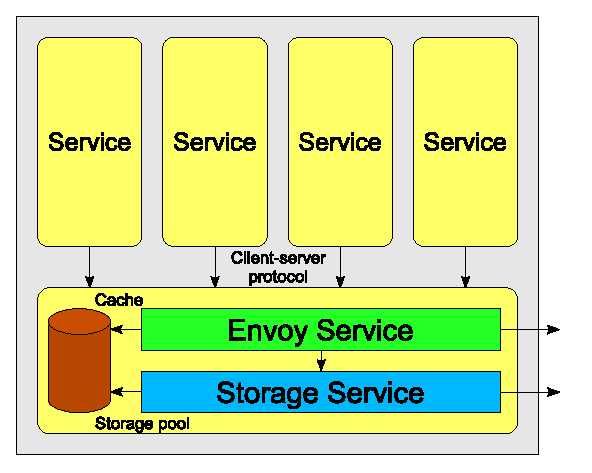
\includegraphics{figures/single-machine}
\caption{Each physical machine has a single administrative VM that hosts the Envoy services. This VM exports a network file system protocol to other service VMs running on the same machine.}
\label{fig:single-machine}
\end{figure}

The file system management processes join a cluster-wide service that is comprised of two primary layers, as illustrated in \prettyref{fig:layers}. Storage is managed by the lower level, which allows a small set of basic file operations on objects. All operations are stateless and the storage service makes no attempt to prevent or manage concurrent requests or to enforce any kind of security policy. Objects are extents of bytes with a small set of attributes.

On top of the storage service is the envoy layer, which builds a hierarchical file system out of objects, coordinates access to files, provides authentication and access control services, manages caching, and exports a standard network file system interface for services to access.

\begin{figure}[tp]
\centering
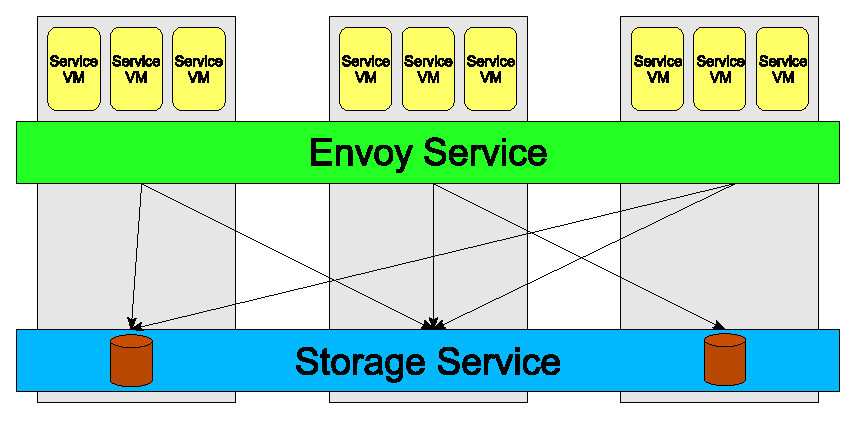
\includegraphics{figures/layers}
\caption{The envoy service coordinates access to provide a single, coherent view of the distributed file system. It relies on the storage service, which provides a repository of objects referenced by unique identifiers.}
\label{fig:layers}
\end{figure}

In the remainder of this section I detail the functionality and requirements of these systems and consider the tradeoffs of various design decisions.

\subsection{Distribution}

\prettyref{fig:client-server} depicts a commonly-used storage arrangement using a series of dedicated file servers to handle the needs of many clients. This architecture is successfully used in many settings and, despite alternatives developed over the years, is still the dominant storage model in practical use.

\begin{figure}[tp]
\centering
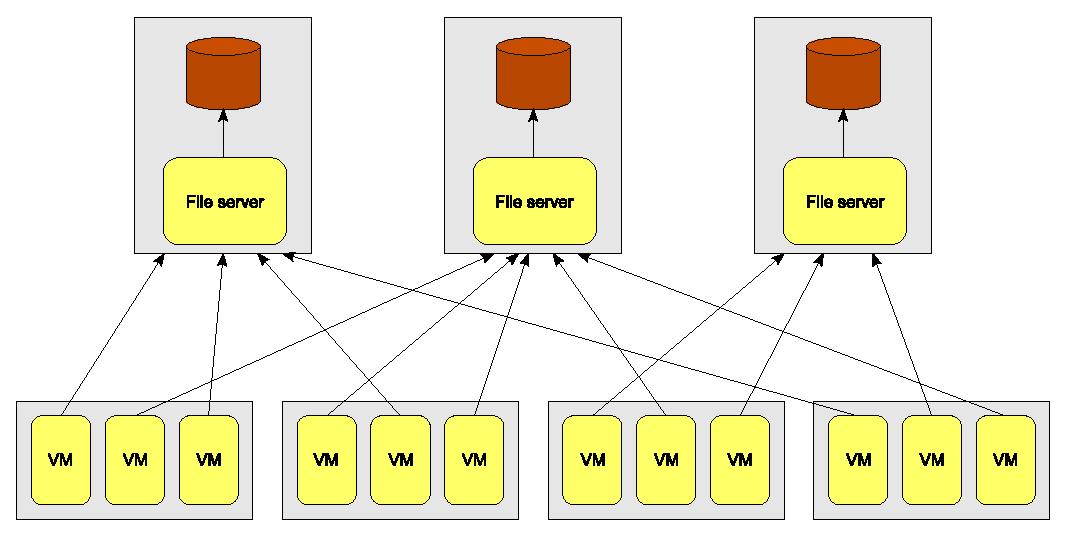
\includegraphics[width=100mm]{figures/client-server}
\caption{A popular storage solution for groups of clients involves a series of dedicated servers. Content on the servers is carefully managed to distributed storage demand and transaction load between the servers.}
\label{fig:client-server}
\end{figure}

The client-server model has obvious flaws when applied to clusters with many transient clients. Data placement decisions must balance space requirements and expected access rates in order to avoid overloading a particular server. Rebalancing---a disruptive and time consuming job---may be necessary in response to added clients, added servers, added disks, variations in client workload, and accumulation of data over time.

With the service cluster model, the problem is made even worse. To make efficient use of increasingly powerful hardware, each physical machine may host many services, each of which requires a boot image as well as access to the data relevant to its intended task. Dividing each machine means that there may be an order of magnitude more virtual machines than physical machines, putting excessive demands on a centralized storage infrastructure \cite{hospodor}. Single-purpose services may also be short lived or vary by time of data, making manual balancing impractical.

The client-server model has not endured as long as it has simply for lack of alternatives, however. It has many strengths that can inform the design of a more distributed architecture. With a single server managing shared data, concurrent access can be managed simply through explicit leases and cache invalidation, centralized caching with synchronous access, or through a lock manager. Whatever the mechanism for resolving conflicts, a centralized server is ideally suited to detecting and responding to concurrent requests because it is the point on the access graph at which all requests converge. The consistency of data that has reached the server is as good as its backing store.

The simplicity of a server is also a virtue. A failstop model for reliability can generally be assumed, backups are relatively straightforward, the server is typically dedicated to a single task or is shared with other trusted services, and the semantics are simple to define in terms of client behavior%
\footnote{NFS versions 2 and 3 have notoriously complicated consistency semantics, but this is almost entirely due to client policies. NFS server semantics are straightforward.}.

The chief faults of a centralized system are the introduction of a single point of failure and the inability to scale beyond the network and disk bandwidth that can be hosted by a single server. While these limits are unacceptable at large scales, they are quite servicable for small groups of clients.

For clients that are sharing data, it is difficult to improve on a centralized server. For sufficiently overlapping data sets, any consistent model will degrade to something resembling a server during periods of contention because all interested clients will have to synchronize their access to the contended bits. A single arbitrator will ultimately oversee each bit of data, whether it is a traditional server, a lease-holding client, or a quorum of cooperating peers.

Sharing cache space is also a benefit of consolidated control of shared data. As the performance gap between disk access and memory access continues to grow, efficient use available cache space becomes increasingly important. Once again, a single centralized cache fails the scalability requirement, but a shared cache for a smaller set of clients with overlapping data needs provides attractive properties. Accessing a cache across a high-speed network is faster than accessing a local disk \cite{dahlin94b}, so in a cluster setting, organizing the aggregate cache around shared access patterns is more valuable than organizing it to localize access. Stated another way, the combined effective cache size of the entire cluster is greater when redundant entries are consolidated through sharing, and maximizing the combined cache size to avoid disk seek penalties is becoming more important than avoiding the network hops that arise from using a shared cache.

While a server cannot handle an unlimited number of clients, it can serve many clients under typical workloads. Scalability matters more at the level of the entire distributed system than when considering individual nodes. In the case of overlapping requests from different clients, a shared cache on a shared server will outperform a series of private servers, despite the overhead of network latency. Given that runtime contention is relatively rare \cite{kistler}, Envoy is designed to localize file ownership when there are no apparent conflicts, but to pick one participant to own files that are shared and act as a server to the others.

This principle of localizing control where possible, but reverting to a simple, well-understood client-server model when sharing is necessary is fundamental to Envoy. It leads to \emph{fate sharing} amoung clients with overlapping interests in the areas of performance, resource usage, and failure recovery. In each case, services with overlapping resource demands cooperate directly with each other and disinterested parties are not involved.

The overall distributed architecture of Envoy is modeled after human-administered systems using client-server file systems. Storage is distributed over a series of servers in an attempt to balance demand (the seperate storage layer handles balancing capacity), but where a human administrator is constrained by practical concerns to using relatively few, well-provisioned servers, an automated system can continue the process of server division and balancing to a much more fine-grained level. Entire images or parts of images that are used exclusively by a single service (or a group of services hosted on a single physical machine) are managed directly by the envoy service on the same machine. Where sharing occurs, the client with the highest demand retains direct control and acts as a proxy for other clients accessing the same storage, thus sharing a cache and avoiding complicated coordination protocols.

\subsection{Storage layer}

Citations: \cite{stein05}, HP trace shows that with caching, most operations that go to disk are writes, and non-sequential operations \cite{ruemmler}, so access patterns are probably less important in the storaage layer than recovery concerns, which pimp for chained declustering and correlated failure \cite{lee96}. Object storage works well and is growing in popularity \cite{factor}. File layout doesn't matter as much behind the cache \cite{stein05}

The objective of the storage layer is to provide a simple, stateless interface for accessing objects. Redundancy to enhance availability and reliability and distribution to balance load is also handled by this part of the system. The storage layer is implemented in two parts, called the top and bottom halves.

The bottom half is implemented in the storage daemon hosted on each physical server. While the storage daemon instances form a collective pool of storage, they do not communicate directly with each other. At the local level, each storage manager is unaware of any global state, and responds blindly to incoming requests from the envoy layer. Instances do not attempt to balance load, resolve conflicting requests, or create redundancy, nor do they monitor which object IDs they considered valid. Instead, they provide a thin, simple storage service for numbered objects with attributes.

To make these servers more useful, the top half of the storage layer is implemented in the envoy daemon. It is responsible for mapping an object ID to the set of storage server instances that host the referent object. Combined with the persistent cache, the storage layer top half provides a simple procedural interface to the storage layer, where objects are named by unique IDs. The top half is responsible for creating and locating replicas, detecting and masking/recovering from failures, allocating new object IDs when needed, and reading and writing data and attributes.

Numerous strategies are available for distributing objects across the cluster. While I discuss some of them here, I only do so with the intent of demonstrating that an independent storage layer is viable and reasonable; many other object storage systems of varying levels of sophistication could be substituted for one I describe and other work has addresses object storage in more detail than I attempt here. The emphasis of this dissertation is on the envoy layer as implemented on top of the object layer.

\subsection{Envoy layer}

The envoy layer forms a file system from the objects provided by the storage layer, coordinating and caching access to the file hierarchy, and exporting a client-server protocol to services that act as clients of the file system. The entire cluster shares a global, hierachical namespace, but clients typically mount a subtree from the hierarchy and treat it as a complete file system.

\subsubsection{Territories}

A single instance of the envoy service runs on each physical machine. The global name hierarchy is divided amoung participating instances in the cluster. When a given instance takes responsibility for some part of the namespace, it is said to \emph{own} a \emph{territory} covering the relevent subtree of the hierarchy. All operations within local territories are served locally and may be cached locally both in memory and in the persistent cache, which is reserved exclusively for territories local to the machine.

This partitioning of the global namespace and the resulting federation of constituent parts is what gives Envoy its name. When clients request operations that stray from the local territories, the requests are handed off to the envoy on the appropriate machine. It follows that each instance must know not only the boundaries of its own territories, but how to find the envoy for neighboring territories, i.e., those that can be reached by a single directory traversal (up or down) from a local territory.

The envoy service is stateful, and tracks not only its territories and neighbors, but the state of all files and directories in use by its client services. When a client navigates beyond the boundaries of a local territory, requests are forwarded directly to the owning envoy. If further navigation moves beyond the neighbor's territories, the neighbor does not forward it to the new envoy, but instead bounces the request back to the originator with the address of the envoy that can answer the request.

Under this system, two envoys maintain a direct relationship with each other only when they are immediate neighbors in territory ownership, or when one is serving requests for a client of the other. It follows that if territories are alloted such that the owner of a territory is also its most active user, traffic on an envoy instance will generally be dominated by its local clients.

Often, the best that can be achieved in a steady-state system is to have the owner of a territory be the envoy driving a plurality of traffic, not a majority. Sometimes this is an inevitible consequence of overlapping client demands, but often some further gerrymandering of the territory boundaries can restore a majority to the local territory. Since the needs of the clients and the needs of the envoys are generally aligned, a practice that in polotics usually serves those in power at the expense of those they represent serves both equally well in file systems.

\subsubsection{Files}\label{sec:directory-format}

Files and directories can be mapped easily to objects as provided by the storage layer. Files are stored as objects with a set of attributes, and directories as files with special semantics and a different interface. Certain special files are stored as normal files with special contents, accessible through the interfaces appropriate to the file types.

Unix file systems are organized around \emph{inodes}, which encapsulate the contents of a file with its attributes, but not with its name. Envoy employs a similar structure, with file contents and attributes seperate from the name hierarchy. Objects also have numeric identifiers like inodes, but it is worth noting that these identifiers can change during the lifetime of a file, so an object ID is not suitable for identifying a file.

Directories are files containing listings of other files. In Envoy, directories are managed at the block level, with each block containing some number of entries. An entry consists of a file name, the object ID that links to its contents and attributes, and a flag indicating the file's copy-on-write status. When this flag is set, the object is considered read-only, and will be cloned before any changes are committed to the file's contents or attributes. This process is completely opaque to clients.

Special files, such as device nodes and symbolic links, are stored as regular files whose contents follow a defined format. For symbolic links, the file contents are the target of the link, for devices they are an ASCII string identifying the major and minor device numbers, etc.

\subsection{Caching}

Citations: Most files in a file system (90\%) are never accessed after being created and as few as 1\% are used daily \cite{gibson98b}, so even a small persistent cache can be effective, and sharing the active files from boot images and the like will probably see heavy overlap: after all, moving only 1,000--10,1000 objects takes 42--77\% of the load with it \cite{klosterman} (reconcile this with \cite{muntz}). Another workload comparison \cite{roselli}. DBMS work also explores the idea of considering the aggregate cache capacity of the client-server system \cite{franklin}. Self-similarity in file systems \cite{gribble}. Speculative execution has been used to mask the latency of distributed file systems \cite{nightengale}, allowing improved performance without sacrificing cache consistency, and approach that compliments ours. Other work on consistency \cite{triantafillou,vilayannur}.

The cache design in a distributed file system must balance the needs for performance, consistency, and durability. While maintaining a coherent view of the file system that is tolerant to software and hardware faults, a cache should reduce latency, increase throughput, and increase overall capacity by reducing the network and disk congestion required by a given amount of activity and freeing input/output channels to absorb additional load.

Enhancing performance is the primary reason for employing a cache in the first place. The growing gap in performance between main memory and disk makes effective cache management critical, as a random disk access is five or six orders of magnitude slower than a similar memory access. Much work has been done exploring different cache replacement strategies, with significant gains to be had when future traffic can be predicted. Unfortunately, the service cluster environment does not provide any insight into the expected access patterns of its constituent services, as one of the purposes of the environment is to support arbitrary services.

In a 2002 interview \cite{spring}, the CEO of Google observed that for seek-intensive workloads, DRAM can be cheaper to deploy than disks. The seek time of a single disk cannot be improved significantly, so increasing overall disk performance generally requires adding redundant spindles. With many mirrored disks, many seeks can proceed in parallel and a random request can be satisfied fastest by the disk whose head position happens to be nearest the requested datum. Because the of the large performance gap, Google found it cheaper and faster to store their entire web search index in DRAM, which can serve many requests quickly, than to create enough replicated disks to handle the same transaction load.

While Google's implementation revolved around an inherently parallel task, it can still inform the design of a cache solution for Envoy. A single, commodity machine cannot hold as much memory as would be required for an index of the web, but by considering the aggregate capacity of a cluster instead of focusing on the capabilities of a single machine, they arrived at the suprising but sensible conclusion that ``it costs less money and it is more efficient to use DRAM as storage as opposed to hard disks''. Finding data in a local cache is ideal, but with a high-speed network connecting machines in a cluster, it is faster to query the cache of another machine than a locally-attached disk \cite{dahlin94b}, suggesting that it would also be prudent for the design of Envoy to consider the combined cache of the cluster as well as the cache of individual nodes.

Envoy is designed to compromise between the competing goals of maximizing local cache hit rates and maximizing the aggregate cache capacity of the cluster. Two design features are particularly relevent to addressing these goals. The first is that all client requests are served synchronously by the envoy service without the aid of a local cache. Instead they rely entirely on the shared cache hosted by the envoy service in its private virtual machine. The local envoy directly services all requests---local and remote---for territories it owns, so the entire cluster caches at most a single copy of a given file.

This could potentially strain the envoy that owns a particularly popular file, as it funnels all traffic for that file to a single node. For light to moderate sharing, this is not an issue, and in practice the envoy will be accessing the file mainly from its cache and can handle significant traffic. For extreme instances of sharing, I argue that services should use explicit network-facing protocols instead of relying on the file system as a \emph{de facto} distributed shared memory system.

The second design feature has a more complex impact on the aggregate cache capacity. Territorial boundaries are drawn along boundaries in the namespace hierarchy, but because of the copy-on-write mechanism in snapshots and file system forking, multiple names may refer to the same underlying storage layer object. This only happens when the object (but not necessary the file) is read-only, so cache consistency needn't be considered, but it does mean that multiple envoys may cache the same underlying object. While this mechanism introduces redundancy in the cluster-wide cache, it also has the potential to consolidate cache entries within a single envoy instance. If multiple services are using different files backed by the same object, they will occupy the same place in the persistent cache as well as the in-memory cache.

Cache utilization is most effective when clients on a single machine use file system images forked from a common root, and the more complete the root image the more likely it is that services will rely on common rather than custom-installed files. This fits nicely with the stated goals of flexible commodity computation, where both the host and the client gain from using the most popular commodity tools. The host by reducing client footprint and increasing capacity, and the client by reducing deployment costs and maximizing performance through increased cache hits.

\subsection{Data paths for typical requests}

To summarize the architecture of Envoy, consider the data paths followed by typical file system requests as depicted in \prettyref{fig:hops}. The best case (retrieval from in-memory cache on the same machine) is designed to be the most common, with extra steps being required in progressively less-common operations until the worst case, where a request travels from a client to the local envoy service, is forwarded to a remote envoy, misses the local cache and is forwarded to a storage server instance where the data is retrieved from disk.

\begin{figure}[tp]
\centering
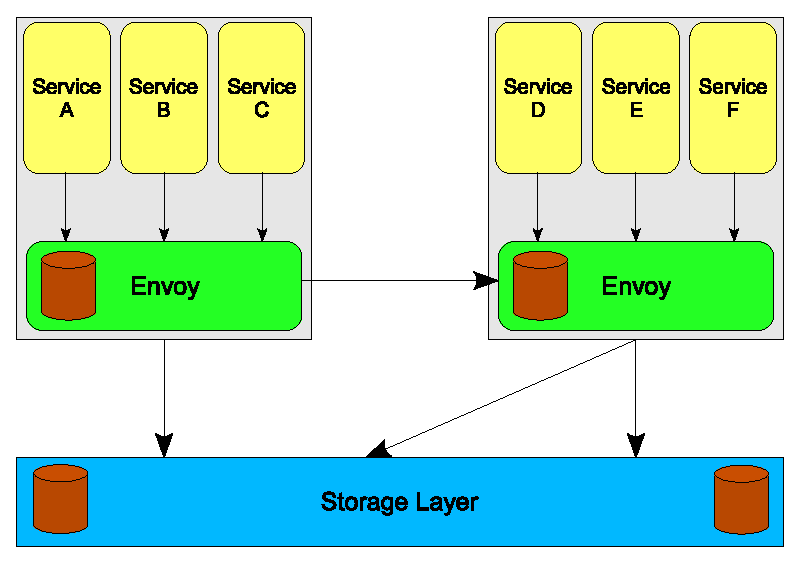
\includegraphics{figures/hops}
\caption{File system requests proceed from service VMs to the local envoy service. A request from a local territory may be filled by the local in-memory cache, the local disk cache, or by a single network hop to a storage server. A request for a foreign territory adds a single network hop in each case, as the local envoy acts as the client to a remote envoy.}
\label{fig:hops}
\end{figure}

\subsubsection{Read operations}\label{sec:data-paths-read}

The best case is a request for hot data in a local territory. In this case, data can be served from the in-memory cache of the local envoy server. With a fully optimized implementation using Xen or a similar VM environment, this data transfer can occur with a single data copy from the cache to a data page, and that page can then be swapped directly to the client VM via page table manipulation. Since the client's OS does not keep a cached copy, that page can likewise be passed on directly to the client application. While my prototype is not this optimized, the design permits a very lightweight operation involving a single data copy and some metadata manipulation.

Warm data from a local territory follows a similar path, prefaced by retrieving the requested data from the local persistent cache (on disk) into the in-memory cache. With large, cheap commodity disks, the persistent cache can easily hold several operating system images and typical application suites. Typical Linux installations occupy no more than a few gigabytes, and even that includes many supporting files that are rarely used and may never be referenced in common service deployments. If services have forked from standard base images as proposed, it is realistic to assume that the entire operating system and standard applications will be available in the local cache hierarchy for a service being deployed on an active node.

When the local cache fails to deliver, the envoy service must retrieve requested data from the storage layer. The top half of the storage layer provides a complete object server catalog, so a request can proceed in a single network hop to the node in the storage layer bottom half that hosts the needed object. For simplicity, the persistent cache holds only complete objects, so an entire object must be transfered before the envoy service can begin fulfilling requests from the local cache. If the object is replicated, the envoy stripes the transfer across the servers, e.g., if there are three replicas, it streams the first third of the file from the first server, the middle from the second server, and so forth.

Operations in territories outside local control add an extra network hop between the local and remote envoys for all operations. The data also bypasses the local cache, so locality of reference does nothing to remove this network penalty. It does offer another optimization opportunity (the data, once received from the network, can be passed to the client application without any further copying) but this is minor compensation for a guaranteed latency penalty.

Fortunately, this penalty need not be too great nor too common. The remote envoy handles the request just as it would one from client local to it, including caching, so referential locality does improve performance from the cold-cache worst case. The target environment is service clusters, too, with high-speed local area networking and unmetered inter-node traffic. Finally, because of the way territories are decided, in a steady state system foreign envoy requests generally imply some degree of sharing. While relatively uncommon in itself, genuine sharing requires \emph{some} form of synchronous network communication to guarantee consistency, so Envoy's goal of reducing synchronous inter-node to cases of either sharing or infrequent access seems a reasonable one.

\subsubsection{Write operations}\label{sec:data-paths-write}

Citation: Transactions, strengths and weaknesses \cite{gray81}.

Write operations are less common than reads, but much of the complexity in file system design comes from supporting them. While a good cache satisfies many read requests from memory quickly and with no correctness concerns (provided coherency is maintained in the case of distributed systems), write operations cached in memory raise concerns about durability. If the server acknowledges the write operation as being complete but has only committed it to an in-memory cache, then there is a window of vulnerability before the data is stored to disk and all metadata updated wherein a system crash could lose data that the client expects to be resilient to crashes. In an isolated client, this may be acceptable as the client will simply be forced to restart from the state that was committed to disk and will generally only lose a boundable amount of work. It is particularly problematic for distributed systems and others with external side-effects, however, where other participants may cue subsequent actions on the premise that a write has been successfully and durably committed to disk. The problem is further exacerbated in a commodity hardware environment where failures are routine.

At the other extreme, one can commit all writes to disk before completing the transaction. This makes it clear to the client when a write operation has been consumated, and it is free to either wait for the acknowledgement or proceed asynchronously with explicit knowledge of the risk it is assuming. While this is a simple and appealing model, it ignores two important realities. The first is that the default action for most commodity operating systems is to cache writes and acknowledge them immediately while delaying the disk write. Changing the expected performance characteristics of a basic operation like writing to disk would not provide a commodity-friendly environment as it would severely affect the perforamnce of many standard tools in a negative way. The second is that most files created are short-lived temporary files that are soon deleted \cite{ousterhout}, so synchronously writing them to disk introduces not only unnecessary latency but also unnecessary disk contention.

Several intermediate possibilities exist. Instead of having write requests proceed directly to the storage layer, the local persistent cache could be used as a staging area, with write requests being committed locally and then forwarded to the storage layer after some delay. This would do little to improve performance, however, as synchronous disk access is slower than synchronous network access, so this would not eliminate the slowest link in the event chain. Specialized hardware with involatile memory could also act as a staging area, giving good write performance while retaining durability. The latter approach violates our goal of using widely-available commodity hardware, however, and neither approach is resilient to hardware faults that result in the entire node failing.

Another approach is to only guarantee synchronous durability when explicitly requested by the client, using the equivalent of the Unix \texttt{fsync()} system call. This matches the semantics of local file systems, and thus what most software is written to assume. It is not without faults, however, as the popularity of high-level scripting languages and middleware frameworks (especially for network services, exactly the types of clients service clusters are designed to support) means the connection between application actions and disk operations is often obscured. Requiring low-level controls to get correct behavior is often an acceptable compromise, but it is rarely ideal.

The solution Envoy employs is based on exploiting the cluster environment. While commodity hardware is expected to fail occasionally, simultaneous failure of multiple machines is still relatively rare, provided that the nodes are sufficiently isolated from each other in terms of power and cooling. Since service clusters are intended for professional hosting environments, it is reasonable to assume that hardware faults occur in isolation. With that assumption, durability is less about committing data to disk and more about rudundancy. A write request is considered final when it is in the memory of all of the storage servers that will eventually commit it to disk. If the envoy server fails, the storage servers are unaffected. If one or more of the storage servers fails before committing the data to disk, the recovery mechanism must restore consistency using the most up-to-date of the replicas. Having storage servers potentially out of sync due to a failed asynchronous write in this scenario is fundamentally no different from having one fail while trying to satisfy a synchronous request. In both cases, the inherent asynchrony of the network means that only the degree of the problem changes.

\section{File system images}

A single, hierarchical namespace unites all the participants in an Envoy cluster, but for management purposes there are two distinct levels. The administrative file tree starts at the root of the namespace and has as its leaves the file system \emph{images} that are normally accessed by clients. Imposing this additional structure in the tree codifies the intended usage pattern, which simplifies administration and allows for some simple but effective optimizations.

\subsection{Security}

Service clusters must accomodate a heterogeneous collection of clients, some of which may trust each other, but most of which will not. To support standard operating systems and tools, Envoy must support familiar semantics, including granting complete control over private images, while also accomodating shared images that grant limited access to various clients.
\note{TODO}

\subsubsection{Enforcement}

Envoy is designed with a fail-stop failure model. This is relatively simple to deal with, but is unrealistic in many environments. Service clusters 

Envoy services run in trusted virtual machines that are administered by the owner of the cluster. Messages from one envoy to another and to storage servers must be authenticated to ensure , either by  
\note{TODO}
\subsubsection{Policy}

Access to images is controlled through \texttt{password} files in the administrative directories. At the time a client mounts an image, its credentials are checked against all password 

\note{TODO}

\subsection{Forks and snapshots}

A few additional rules simplify management. The root of the namespace is always writable, as are all administrative directories, i.e., those that are not descendents of a directory called \current or one of its numbered snapshots. Snapshots are always immutable

\subsection{Deleting snapshots}

Storage space is cheap and plentiful, and systems such as Venti are designed to keep a complete history of all files ever created \cite{quinlan}. This may be appropriate for some workstation environments, where the increase in storage capacity can outpace typical data creation rates, but deleting files permanently is still a necessity for many other users. In service clusters, users are charged according to the resources they use, so they must have the flexibility to completely remove old files. Also, when clients leave a particular service cluster, the owner may wish to reclaim the space for future use, as there is little incentive to keeping it around on behalf of a client that is no longer paying. Also, concern for privacy and complience with data retention laws may require data to be completely removed.

Backups in Envoy are done through snapshot operations, and anything created and deleted in the window between two successive snapshots is no longer accessible anywhere so it is deleted immediately (with an exception described in \prettyref{sec:hard-links}). This is easily detected through the copy-on-write mechanism, which identifies all files that were created since the most recent snapshot. All files with copy-on-write flags (either explicit in a directory link or implicit through an ancestor's link) are backed by objects referenced by one or more read-only snapshots, so envoys never delete these objects when their corresponding files are deleted.

The problem comes when trying to delete old snapshots, as it can be difficult to determine which storage objects are used only by the files in a given snapshot.

One obvious solution would be to implement reference counting in the storage layer. This has the advantages of simplicity, accuracy, and immediacy. The main disadvantage is that it puts the performance burden in the wrong place: every time a directory object is cloned (an frequent operation after a snapshot as the copy-on-write mechanism supports write requests) the reference count for all objects in that directory would need to be incremented. This would require clone operations to be implemented in the envoy layer which can locate all object replicas, or the bottom half of the storage layer (where clones are implemented) would need to be aware of the topology of the entire storage layer, a requirement currently confined to the top half. In either case, a lot of extra traffic would be generated to support an operation that is relatively infrequent and not timing critical.

The copy-on-write mechanism in Envoy is similar to the one I implemented while working on Parallax \cite{warfield}, as is the problem of deleting snapshots. The problem was simpler in Parallax, however, which uses a copy-on-write radix tree to map logical blocks to physical blocks in a virtual block device. The virtual block numbers do not change between snapshots, so comparing the physical blocks mapped to by two successive snapshots reveals which blocks from the first were unlinked during the lifetime of the second.

With Envoy and its hierarchical file tree, the problem becomes more complex. Comparing two successive snapshots is no longer straightforward, because files and directories can be renamed. The virtual block IDs that are static in Parallax are replaced by variable names in Envoy, making the process of comparing two snapshots more difficult. Supporting hard links makes it even more difficult to define a one-to-one correspondence between object references in two successive snapshots.

This potentially messy problem can easily be solved by brute force. Instead of imposing extra runtime overhead for normal file operations or attempting to walk two file systems and identify matching files within them, it is simple and practical to gather a complete list of objects referenced by an image. Using 64-bit object IDs, such a list would take 8 megabytes for every million files. In a 1999 study of workstations at Microsoft, Douceur and Bolosky found an average of 13,309 files over 10,568 machines, with the subset running NTFS (the newest file system studied and the one with the largest average number of files) averaging 24,229 files over 3332 machines \cite{douceur99}. This number will no doubt continue to grow, but anecdotal tests found the number still in the low millions for typical, modern Linux desktop installations.

Just as high-level languages are worth using despite being slower and using more memory than lower-level languages, I consider the simplicity of gathering a complete list of objects and sorting it to outweigh any potential performance loss compared to a more sophisticated but more complex approach. For problems like this one, it is not even the relative performance or storage requirement that is salient, but the absolute size: deleting snapshots is not a critical path operation and for typical image sizes the brute force approach is cheap enough that no amount of optimization would be worth more than a very small complexity increase (Amdahl's law \cite{amdahl} is relevant here, but the ability to execute the operation asynchronously makes any (reasonable) cost even less important).

A sorted file with all object IDs referenced in the snapshot can easily be stored in the administrative directory that contains the image. To delete a snapshot, the objects of it and its immediate successor and predecessor are compared in order. Each object that appears in the snapshot but disappears in the successor can be safely deleted from the storage layer. To make it safe and resilient to crashes, the envoy service ensures that no clients are currently accessing the snapshot, then it unlinks the root of the image first, and deletes the list of object IDs last. At recovery time, an object ID file found without a corresponding image indicates that a crash occurred before the operation completed, and it can be safely restarted. The image itself isn't necessary at this stage, and as long as the cleanup process can tolerage objects having already been deleted, it can work entirely from the object lists.

The only other complication in this process is image forks, where multiple successors may exist for a single snapshot. Forking an image does not directly affect the snapshot used as the starting point, so the easiest way to detect forks it to log them. The log is consulted before any snapshot delete attempt, and deleting images that have more than one immediate successor is not permitted.

A few other corner cases are worth mentioning. The current version of an image can be deleted using the same procedure, but it must be made read-only or client access must be disallowed before gathering the list of object IDs (note that access is normally only forbidden when deleting starts, as the catalogs of predecessors and successors must be assembled as well as those of images marked for deleting). Otherwise, the normal procedure suffices, with the successor object catalog taken to be empty. The log of image forks also needs to account for deletes, so that entire trees of images can eventually be pruned back to the root if desired.

\section{Dynamic territory management}

The Envoy file system model is based on the idea of presenting a single, large file tree connecting arbitrary images, but providing incentives to use it in ways that can be exploited to provide good performance and scalability. The service cluster model makes it simple to isolate control of the file system from the clients who use it, while still keeping synchronization logic and caching on the same machine most of the time. Providing a global namespace gives a great deal of flexibility, but inferring usage patterns and co-locating ownership of branches of the tree with the clients that use them yields short data paths and good performance.

\subsection{Design principles}

A variety of approaches to distributing territory ownership are possible, and only a realistic usage model drawn from empirical study of real-world deployments can accurately inform optimum choices. Lacking that, territory management in Envoy is designed around a few principles:

\begin{itemize}
\item Optimizing long-term patterns is more important than following short-term trends. High-speed switched networks minimize the penalty for serving a request from a remote envoy compared to handling it on the client's envoy, and the growing gap between memory and disk performance makes flushing the cache with a territory move continually more expensive. Based on this and on the past success of client-server file systems, Envoy favors slow evolution of the namespace topology to capture steady-state client behavior.

\item Simplicity is a virtue. This applies to the runtime behavior of the system as well as the algorithms and implementations that drive it. For debugging, recovery, and runtime analysis, territories with simple boundaries that do not change frequently are prefered. Painting the namespace tree in broad strokes makes it easier for humans to comprehend and analyze, minimizes perverse cases that can threaten correctness and the success of recovery operations, and makes global logging of changes practical. With this in mind, Envoy favors using a few territory divisions to give good results over making many divisions in an attempt to approach optimal results.
\end{itemize}

\subsection{Special cases}

Many systems use leases to coordinate access to file system objects as a form of token passing. When a client wants to access a file, it must first gain control of the file, and it must transfer control to a second client before it can operate on the same file. This may be limited to write operations, allowing a window of delay before updates are visible to other clients, but in either case the transfer of control happens in real time before a request can be satisfied. While these operations can be optimized, fundamentally they operate on a pessimistic model similar to mutex locks in shared memory schemes.

Territories in Envoy are analogous to leases and token systems in many ways, but they are based on an optimistic model where large groups of files can be granted to an owner on the assumption that sharing is uncommon. Every request from a client can be processed immediately either by the client's envoy or by a direct, already-established link to the owner, with complete access to the owner's cache. In this way it is more like a set of manually configured servers that are dispersed throughout the cluster than a set of lease-holding clients with equal claim on an object. Performance is best when the server is on the same machine as the client, but it is not bad when an extra link is introduced.

The decision to cede all or part of a territory to another envoy is always made by the current owner. While a client's envoy may be able to recognize the client's ongoing demand for a particular region of the file tree, only the envoy that manages it can account for all clients that are accessing it and act based on complete information. Transfers are always driven by the parent of the root of the branch being transferred, but the parent only initiates a transfer when the owner of the branch requests it. This leads to the first special case in territory realignment: when a territory is dormant, it is ceded to its parent. Dormancy is determined through the general mechanism described below, but this is highlighted as a special case because no other envoy can detect a territory that has fallen out of use. Territories are also ceded when an envoy is shutting down.

Another special case is based on the expectation that most images (especially those used as boot images) will be used by only a single client: when a client mounts an image that is not in active use, the image is immediately ceded to that client's envoy. The first client to mount an image may not be the one that expects to use it the most, but it is more likely to do so than the owner of the parent, which may have no interest at all in the image. For services with no sharing, this heuristic by itself is sufficient to completely localize non-administrative traffic. This is also an example of how imposing a little structure on the file tree can not only simplify administration, but also improve performance.

\subsection{Changes based on sharing}

The interesting case is when sharing occurs within an image. The envoy tries to find the simplest change that will improve 

\section{Recovery}



\section{Summary}

\subsection{Desirable properties that the envoy model achieves}
\begin{itemize}
\item distribute only when there's a reason; favor centralization when practical
\item perfectly consistent persistent caching without constant refresh checks
\item local impact---heavy users bear most of the load, non-users none of it
\item serve from local machine cache when uncontended, NFS-like when shared: requests never require topology changes
\item in steady state, coordination based on actual contention, not potential contention
\item simple security model that maps well to familiar Unix semantics
\item private images act like local images, shared images scale gracefully
\end{itemize}

Lease migrations work to optimize traffic patterns in the long term, but migrations are just that: an optimization. They only help when there is heavy traffic or a long-term pattern, where caching can come into play. Frequent changes thrash the cache and disrupt normal operations. Migrations require coordination between envoys and may require halting normal file system traffic. We want infrequent lease changes that give good long-term behavior rather than frequent changes that try to chase short-term trends. Since latency is short in a cluster, we don't lose all that much by going to a remote envoy for requests: this is a lot like conventional NFS servers now which seem to do just fine. One consequence of this is that lease migration operations can be straightforward and obvious without heavy optimization, while still not hurting the overall system too much (Amdhal's law).

\chapter{The Envoy Prototype}

\section{Scope and design coverage}

\section{The 9p protocol}

Clients access Envoy using a client-server file system protocol between the virtual machine of the client and that of the envoy service. While a custom protocol would offer the greatest flexibility, it would also make the implementation considerably more complicated and would have little value in demonstrating the viability of the design.

With Linux as the client operating system of choice, a few prominent options were available:

\begin{description}
\item[NFS version 3] The NFS protocol is popular, simple, well-understood, and has a robust implementation. Most of the complexity is implemented in the client drivers, so servers can be quite simple. I also had experience with the protocol after implemented a stackable, copy-on-write file system (CoWNFS) for the XenoServers deployment project \cite{kotsovinos}.

For user mode servers generally and Envoy in particular, however, the stateless model of NFS complicates implementation. File handles assigned by the server and given to the client are expected to be immutable and always available (there are no explicit open and close operations), making it difficult to maintain pairings between active files and the envoy instances that own them. With transparent copy-on-write, these handles must either be cached indefinately or inherently tied to the name of the file. Changing territory boundaries makes caching impractical, and allowing for higher-level directories to be renamed makes the latter difficult to make robust.

Security under NFSv3 is based on Unix user and group IDs, which proves to be an inflexible mechanism when diverse clients become involved. The ID space must be shared between clients that share file systems, or the server must provide a mapping service to reconcile the differences. While not an insurmountable problem, this can get unnecessarily complicated when a client mounts multiple file system images, many clients share some images, and parts of those images are forked from standard base images.

The caching model of NFS is entirely under the control of the client driver, which generally sends frequent \texttt{stat} requests to check if its cache is still current. Write operations are generally asynchronous, however, and the lack of control would have defeated the cache coherency guarantees that Envoy seeks to achieve. Caching at the client level would also prevent consolidation of duplicate caches as the physical machine level, another of the aims of the Envoy design.

\item[NFS version 4] The most recent update to NFS addresses many of these concerns by introducing a stateful model and using leases to manage client caching. These client delegations could work well with Envoy, allowing private files to be cached by the client and shared files to be held back and cached by the envoy. More flexible file handles and explicit state management also a better match. NFSv4 would be an attractive candidate for a future implementation, but at the time the Envoy prototype implementation was started, it was still relatively immature and the supporting tools were complicated to use and poorly documented.

\item[AFS] The Andrew File System is another popular client-server system with a mature implementation. It employs persistent caching at the client, which is a poor fit for the Envoy model, and it is not intended as a general-purpose protocol for implementing custom servers.

\item[FUSE] The FUSE driver and tools support custom userspace file systems under Linux. The FUSE interface is also modeled after the Linux VFS interface and exposes some of its complexity, but the main point against FUSE for Envoy is that it is not a network-facing protocol, so a userspace tool for the client would be required that would in turn connect to the envoy service across the virtual network device. Besides adding an unnecessary layer of indirection, this would complicate using Envoy as a root file system.

\item[9p] The Envoy prototype is implemented using the 9p protocol from Plan~9, which has been ported to Linux with some extensions to better support Unix semantics. The 9p protocol is simple and message based with no client-side caching (though the developers have indicated plans for an optional, parameterized cache in the future), symbolic user names, and stateful file management.
\end{description}


\section{Synchronization}

\section{Storage service}

Storage instances are stateless and unaware of higher-level semantics with two exceptions:

\begin{enumerate}
\item Each storage instance can respond to a reservation request, which returns a range of object IDs that have not been used or allocated on that particular instance.
\item The \emph{clone} operation, which copies an object from one given ID to another, will expect objects whose attributes indicate that they are directories to follow a particular format (described in \prettyref{sec:directory-format}) and will set the copy-on-write flags within each block as it copies the object.
\end{enumerate}

Neither of these functions is essential for implementation in the storage layer. The first could easily be performed by a different service (such as an elected instance of the envoy service) and the second is merely a performance optimization. Both are convenient to implement in the storage layer, however, so they are there in the prototype.

\section{Envoy service}

Having examined the high-level architecture of the Envoy file system, I next turn to a more detailed discussion of how specific operations are served. This includes basic file operations and navigation between envoy instances, the copy-on-write mechanism behind the fork and snapshot operations, coordination of state during territory boundary realignment, security considerations, and the procedure for deleting file system images.

For operations that require the synchronous cooperation of multiple envoy instances, dependency cycles and deadlock become a concern. To minimize these issues, Envoy is designed with a top-down locking protocol where synchronous operations only directly involve immediate neighbors in the tree of territories, and owners of territories closer to the root always initiate and coordinate transactions with those lower in the tree. While operations with wide-ranging impact may require communicating with every node in the cluster, they never require a cycle in the connectivity graph and are not prone to distributed deadlock.

\subsection{Freezing and thawing}

Synchronization at the object level is governed by an important invariant: an object in the system may be referred to by exactly one name in the hierarchical namespace, or it must be read-only. The storage layer makes no attempt to detect or enforce the read-only case, so it is left to the envoy layer to ensure that this invariant is preserved. To make this straightforward, objects can transition from being writable to read-only, but they can never go back. Note that this refers only to objects in the storage layer, not to the access control of file system objects.

The same invariant makes cache management simple: the envoy that owns a given territory can cache it without any invalidation concerns, and read-only objects can be safely cached at any number of envoy nodes without fear of interference. Objects in the cache become invalid only when a territory boundary changes. Objects that are part of ceded territory are not explicitly flushed from the cache; keeping them active helps in two cases: a read-only object may still be referenced by another name in a local territory, and the cache entry (in-memory or on-disk) may still be useful if a file backed by that object is later returned to local control. In the latter case the object must be verified to match the version in the storage layer, but this can be done with a lightweight metadata comparison.

The single mutable/multiple immutable dichotomy in the storage layer is tracked in the envoy layer through the copy-on-write flag in directory entries. The immutable property is not directly assigned to objects, but instead is imbued by the link from directory to file object. Furthermore, when the immutable object is itself a directory, the property is applied recursively to all of its children, overriding the individual copy-on-write flag in the link to each child. To be regarded as mutable, an object must be reachable by a path from the root of the global namespace to the directory entry linking to the object without traversing any copy-on-write flags that are set.

One immediate consequence of this is that taking a read-only snapshot of a directory and its descendents requires only setting the copy-on-write flag in the link to it, an operation known as \emph{freezing}. Once a directory or file is frozen, the storage layer objects that back the branch rooted at that point are considered immutable. To simplify bookkeeping, this operation is only performed from the root of client images when a snapshot operation is requested. The benefits gained from this restriction and an exception to it are discussed in \prettyref{sec:hard-links}.

The complementary operation is called \emph{thawing}. While the freeze operation works at the root of a subtree and affects it in its entirety, thawing aims to leave as small a footprint as possible; it is always performed with the goal of modifying a particular file. To thaw a file, the owning envoy starts walking up the line of its ancestors until it finds one that is already thawed. As the root of the namespace cannot be frozen (one can consider it as having a single, implicit link from the envoy service itself, but there is no mechanism provided to set the copy-on-write flag on this implicit link), this search is guaranteed to succeed. From there the envoy walks back to the target file, \emph{cloning} intermediate directories as it goes. In addition to making a copy of the directory as its name implies, cloning sets the copy-on-write flag of every directory entry in the copy, effectively transferring the copy-on-write property from the single link leading into the directory to all the links leading out of the directory. The implicit property that each child inherited becomes explicit after being passed down a generation. After thawing each directory for mutability, the parent is updated to reflect both the new object ID and the cleared flag. Eventually the intended target itself (be it file or directory) is cloned, its immediate parent link updated, and the file is fully thawed.

Thawing resembles the procedure for modifying a value in a tree in a functional language. In addition to changing the value itself, the path from that item to the root of the tree must be copied if the item is to be reachable from the root. In the thawing operation, it is only the root of the immutable subtree in which the item resides that must be copied. While the analagous procedure in a functional language copies everything exactly except for the path being changed, the thaw operation must clear the copy-on-write flag as it goes, and thus must push it down from parent link to sibling links at each level in order to preserve the immutable status of the unaffected branches.

The prototype clones an entire object, but it could be optimized to store deltas or otherwise compress changes, especially in directories and other metadata \cite{soules}.

\subsection{Read operations}

Most basic file and directory operations have a straightforward implementation. The need to cross territory boundaries makes some more complex, however, as they must coordinate with remote envoys to complete.

\subsubsection{Reading files and attributes}

The most straightforward operations are \texttt{read} and \texttt{stat}, which read the data and metadata of files, respectively. These requests can be filled using the data paths described in \prettyref{sec:data-paths-read}. The only complication involved is handling the \texttt{atime} attributed, which tracks the last time the data from a file was accessed by a \texttt{read} or \texttt{write} operation. Read operations always proceed through a single envoy, so this attribute can be tracked accurately: the envoy can send a message with the timestamp (to ensure that it is consistently applied to all replicas, even if all clocks are not in sync or network latencies between the different storage servers vary) to all replicas in the storage layer which can then update the attribute.

The intended meaning of the \texttt{atime} attribute becomes obscured when applied to frozen files, however. Since attributes are part of the object, akin to \texttt{inodes} in traditional Unix file systems, changing the attribute will affect all files that are backed by that same object. Those instances may be in read-only snapshots of the same file system image, or in common files available in an unrelated file system image. In the former case, the read-only property of the snapshot is broken, and in the latter case the isolation of the two images is compromized. Updating the \texttt{atime} attribute would give an unrelated client using the same prepackaged file system image the ability to losely track file accesses, which could represent a security risk.

Accurately tracking the \texttt{atime} attribute is problematic with frozen files, and if it is only updated on some files (which may change over time as successive snapshots are taken), it is too unreliable to be useful. It also generates network and disk traffic for every read, even those that can be satisfied from the cache. For these reason, the \texttt{atime} attribute is present in Envoy for compatibility, but it effectively mirrors the modified time attribute.

\subsubsection{Reading from directories}\label{sec:walk-cache}

Reading from directories introduces two complications. The first---that successive \texttt{readdir} requests require state that must be transmitted from the client each time or transferred to another envoy when territories are realigned---is just an implementation issue. The second---that a directory may span multiple territories---requires the cooperation of all affected envoys. The list of contents for a single directory is considered an atomic unit when drawing territory boundaries, but the files and directories named may be remote. If the client-server protocol used to export the file system to a service only requests names, then the implementation footprint resembles that of file reads. If the response includes attributes as well---as with 9p---additional requests must be forwarded to the respective envoys for all files that are across a boundary in order to ensure consistent results. These requests are sent directly by the owning envoy, so if the client is remote, \texttt{readdir} may require the cooperation of three or more envoys to complete a single request. When gathering file attributes, the envoy that owns the directory sends requests directly to the file owners, resulting in a star topology with the directory owner as the central node. An additional link from the client's envoy is necessary if the directory is remotely owned.

Multi-step directory navigation can also create a star pattern of requests, but they always center around the client's local envoy. Navigating down a series of directories---an operation called \texttt{walk} in 9p---may involve crossing a territory boundary at each step in the extreme case. Because an envoy confines itself to knowledge of its local territories and their immediate boundaries, it cannot always predict the endpoint envoy for a navigation. Even if it could, intermediate steps must always be taken to allow permission checking at each level. When a remote territory must be consulted, the client's envoy forwards all remaining steps in the \texttt{walk} to the remote owner, which proceeds as far as it can with the navigation. It may return one of three results: if the result is successfully completed, the two envoys store any state necessary to handle future requests; if the result is a failure, an appropriate error code is returned; if the navigation reaches another territory boundary, the partial result comes back along with a pointer to the envoy that must be consulted to continue the navigation. The client's envoy then repeats the procedure with the remaining navigation steps.

Because these operations are all asynchronous, and because the navigated directories may be owned by remote envoys that are not even neighbors to the client's envoy, \texttt{walk} may encounter transient failures. Between the time that one remote envoy returns instructions for forwarding the remainder of a request, the target territory may migrate to a new owner and the request will fail. Because the envoy that sent the forwarding instructions was an immediate neighbor of the target, its information must have been correct at the time, and careful coordination can ensure that by the time the target bounces the request back with a failure notice, the referrer knows of the change to its immediate neighborhood. The solution is simply to restart the request from the beginning, which will also correct the client's envoy for the cases of a directory being deleted or renamed.

Generally, having territory boundaries closely aligned with demand benefits everyone, but if multi-step directory navigations are frequent, their performance will be hurt by frequent boundary crossing. Caching \texttt{walk} results can be done safely with a few precautions. First note that a navigation that succeeds one time and fails another implies one of three things: one of the steps was deleted or renamed, permissions changed somewhere, or a different user requested the navigation. The prototype caches \texttt{walk} results keyed by the path traversed and the user that requested it. With the assumption that directory renames and permission changes are uncommon (particularly across boundaries determined by locality of reference---I expect these changes to be most common in a region being actively modified by a single player, not in higher-level directories whose descendents are in active use by different clients), envoys broadcast notification of such changes down the hierarchy when they occur, invalidating cached navigation results. The notification of permission changes is treated as a special case of directory renaming for cache invalidation purposes, as discussed in \prettyref{sec:rename-operation}.

Attributes at the endpoint of the navigation are always confirmed directly with the owner, as are all of the final steps that occurred on territory owned by that same envoy. With a hot cache, multi-step directory navigations are satisfied from the cache of the client's envoy and a single step to the envoy hosting the target of the navigation.

\subsection{Write operations}

\subsubsection{Writing data and attributes}

Like the corresponding read operations, writes to files and changes to file metadata are largely a matter of directing the request to the appropriate envoy. The first change to a file since a snapshot or fork will first require the file to be thawed, but subsequent changes can be made directly to the local cache entries and propogated to all replicas in the storage layer. As discussed in \prettyref{sec:data-paths-write}, changes are considered complete when they have been received by all storage servers, but not necessarily commited to stable storage.

To ensure consistent time stamps, the modification time is determined by the envoy that owns the file and transmitted to the storage layer along with the data being written. While the clocks of machines within a cluster can be synchronized within reasonable bounds, network latencies and variations in storage server load levels would make it difficult to rely on strict synchronization for consistent timestamps. The envoy is a natural location for deciding on the canonical time for its territories.

Thawing a file requires walking back in the file tree until an already-thawed directory is found. To bound the complexity of this procedure and to avoid deadlocks, the root of every local territory is always thawed unless it is part of a read-only snapshot image. While thawing may require cloning multiple levels of the directory hierarchy, this confines the direct impact to a single envoy. It also preserves the top-down rule for synchronous inter-envoy operations by preventing an envoy from demanding a bilateral change from its parent in the tree of territory ownership.

\subsubsection{Deleting files}

The \texttt{inode}-like disconnect between directories and the files they name means that one envoy may own a territory consisting of a single file, while another envoy owns the directory containing that file. Most operations involve either the file itself or the directory, but not both, so it is obvious which envoy should serve the request. Removing a file or directory is a case where the possibility of divided ownership complicates the implementation.

Deleting a file affects both envoys in this case, but the operation needs to appear atomic to clients. The normal rule in Envoy is that the parent should drive bilateral operations, meaning in this case that the owner of the directory should coordinate the removal with the owner of the file. This is a mismatch with 9p, where removal is an operation initiated on a file, not on the directory that contains it.

A higher-level consideration ultimately drives the design of the delete operation, however. Removal can only succeed on files or empty directories, so an envoy that owns the target of a successful delete will have nothing left to own afterward. Instead of trying to atomically coordinate a multi-step the operation between two envoys, the parent instead revokes ownership of the child from its envoy and reclaims it before proceeding.

Since 9p initiates removal with the file to be deleted and not its containing directory, this requires a minor slight-of-hand to maintain the top-down coordination rule. A \texttt{nominate} request is sent from the file's envoy to the that of the parent directory, requesting that it reclaim the removal target. Since \texttt{nominate} operations are implemented strictly in terms of names (not 9p file handles) this request cannot trigger a deadlock, and the remove transaction running on the child envoy effectively becomes a passive observer while control of the territory is transferred. After the transfer is complete, the envoy aborts the transaction and starts it over. Since the file is no longer local, the envoy will either forward the request (if it happens to be the client's local envoy) or reject it, forcing the client's envoy to redirect it to the new owner. \texttt{nominate} requests do not return until all state has been transferred, so the restarted transaction can proceed immediately.

Deletes happen in four basic steps. The first checks that the file is a suitable candidate for deletion, namely that it is a file or an empty directory. The second verifies that the client has permission to remove it from the parent directory, and the third actually removes it. In the case where the territory ownership must change, the envoy owning the file can complete the first step, but it does not know if the second step will succeed and blindly proceeds to initiate the transfer of control. This could cause unnecesary activity if the permission check fails, but in practice the Linux driver used in the prototype does an explicit check before making the delete request, so the possibility of failure is remote: it would indicate an uncommon race condition and does not compromise the correctness of the operation even then.

The fourth step in deleting a file is to actually delete the object that backs it and reclaim the storage space. This is simple enough to do, but deciding when to do it is slightly more complicated. An object can only be deleted when no more names link to it, and to support Unix semantics it should also be preserved until all clients accessing it have closed the file. The former case is easy to detect: if the link to the file was marked as copy-on-write, it shares a link with at least one snapshot and should not be removed. Otherwise, it was created or cloned in the current image since the most recent snapshot and can be safely removed.

To support familiar Unix semantics, the envoy instance strips waits until all file handles are closed before deleting the file. 9p is stateful, so this is straightforward, but it does create a few corner cases that must be dealt with. A new file with the same name could be created, so the envoy cannot continue to track the object by its former name. Without a name the file does not belong to any territory, so it becomes an orphan. Opening a file and deleting it is often done to provide a temporary scratch file that will delete itself if the process dies, but it may still be long-lived. The envoy must still be prepared to thaw it if it was frozen at delete time, migrate it to another envoy in response to demand or to the owning envoy shutting down, and delete the storage layer object even in the event of a failure. The prototype does not address all of these issues, but it does support arbitrary use of the file until the last file handle is closed, at which point the object is deleted from the storage layer if appropriate.

\subsubsection{Renaming files}\label{sec:rename-operation}

Renaming a file exposes the same coordination issues as deleting a file. In 9p a rename request is part of a \texttt{wstat} request, which treats the file name as a property of the file object rather than of the directory that contains it. With rename the issue is even worse than with delete, because up to three objects and three envoys may be involved: one owning the directory, one owning the file to be renamed, and the third owning an old file with the target name that will be implicitly deleted when the rename completes. To further complicate the issue, Unix programs assume that rename-with-delete will complete atomically. Note that the original 9p protocol does not support this (it calls for a failure if the target name is already in use) but the Linux implementation does support this arrangement, and many clients demand it.

As with delete, the prototype simplifies the problem by consolidating ownership of all participanting objects onto a single envoy before making any changes. Unlike the delete case, the renamed file exists afterward and may be a non-empty directory. If it was owned by a different envoy before, that envoy probably drives most of the traffic to it and annexing it into the parent territory may be a poor move for matching ownership with usage. One solution would be to transfer control back to the original owner after the rename completes. It would have to revalidate some cache entries, but they would still be mostly unchanged, and even the in-memory cache would still be usable after a single metadata check on each file. A second possibility would be to engineer a distributed version of rename for these cases, driven by the parent (as with all synchronous operations) and handling transient failures appropriately. A third approach (the simplest and the one taken by the prototype) is to assume that such renames are rare and do nothing. Correct behavior is still maintained, and eventually traffic patterns will force the owner to cede the territory once again if appropriate.

Renames of directories present another difficulty that cannot be safely ignored. Territory boundaries are all managed using directory and file names, so renaming a directory that is ancestor to other territories throws management state out of sync. On the assumption that renaming high-level directories is relatively rare, the prototype handles them by propogating rename events from parent territory to child and from owner envoy to client envoy when they happen, rather than trying to assign immutable aliases for directories or some other similar scheme. Minor overhead in the rare case is usually preferable to complexity in every case.

In addition to updating territory and file handle names, these tree-traversing rename messages flush the walk cache described in \prettyref{sec:walk-cache}.  While a more fine-grained invalidation could be implemented, in practice an occasional flush has very little affect on performance, and it offers a mechanism for solving another problem. As a special case, this message can be used to rename a directory to the same name, forcing a recursive flush of the walk cache but not changing anything else. This is useful when directory ownership or attributes change, and walk operation results that have been cached may no longer be valid. Since this is expected to be rare, it forces a broadcast down the name hierarchy when it happens, rather than forcing checks whenever the walk cache is consulted.

\subsubsection{Hard links}\label{sec:hard-links}

Unix file systems allow multiple names to refer to the same file. While symbolic links merely contain the name of their target, hard links allow multiple links from directories to resolve to the same \texttt{inode}. File operations are coordinated internally with reference to the \texttt{inode}, not the file path, so handling concurrent access is no different than if the clients all opened the same file through the same name. Because \texttt{inode} numbers are only meaningful in the context of a file system, hard links are not permitted across file system mount points. This mechanism is widely used both for aliasing, where two names are given to the same file, and as a way of moving a file without copying it, where the original name is unlinked after the alias has been created. 9p does not support hard links, but the Linux extensions to it do.

While Envoy's structure of names and object IDs resembles the Unix system of file paths and \texttt{inodes}, it does not behave quite the same way. Access coordination in Envoy is done with reference to file names, not storage layer object IDs. When the latter are shared, the objects are assumed to be read-only and can be cached freely on different nodes with no attempt to synchronize access. Different references to the same object ID, even within the same file system image, may be split into different territories and owned by different envoy instances.

For this reason, Envoy offers only partial support for hard links; a file must be frozen before additional names can be linked to it. If futures changes are made to the file through any of its references, the changed versions will be thawed independently and will diverge.

The implementation of the hard link operation is also unique in that the client's envoy intercepts the request before passing it on to the owning envoy if the link is being created in a foreign territory. The Linux extensions to 9p implement hard links by walking to the target of the link, then creating the new link as a file with a special extended attribute containing the file handle of the referent. The file handle state is only available to the client's envoy, so it uses the handle to freeze the target file (if necessary) and rewrites the request to include the object ID instead of the file handle. The envoy (remote or local) can then link the new name to the object.

\subsection{Modifying territory ownership}

Could use leases \cite{gray89}.

Misaligned boundaries do not prevent correct behavior, nor do they introduce a heavy performance penalty. The algorithms to trigger changes are designed to promote good long-term layout choices based on steady-state traffic patterns. Cache effects penalize excessive changes, while the low network latency in a cluster environment reduces the cost of relying on a remote envoy even when local ownership would be preferable. In centralized server systems, all file access is routed across a high-speed LAN to a server with many clients. In Envoy, this pattern is also quite servicable, even when it is not ideal, and Envoy is designed to favor gradual, long-term changes over a quick response in short-term traffic patterns.

Realigning territories requires careful coordination between multiple envoys. In addition to agreeing on new boundaries, state related to active file handles has to be migrated and updated. This includes both the territory owner's state and that of the envoys representing clients, which need to be directed to the new owner. Inflight operations---those that have been initiated by a client but not completed---must also continue and succeed despite concurrent territory changes.

The prototype is designed to make territory migration simple and clear. Performance for infrequent operations has little bearing on the overall performance of the system \cite{amdahl}, and I consider simplicity and an increased chance of correct behavior to be more important in a complex operation of a distributed system (especially a prototype) than optimal performance.

Like other operations involving multiple envoy instances, territory migration is driven by the owner of the parent territory, as illustrated in \prettyref{fig:grant-topdown}. If an envoy wants to merge a territory with its parent, or transfer it to another specific envoy, it sends a \texttt{nominate} request to the parent, giving the root path of the territory and the envoy to which it should be transferred. If a territory owner wants to cede part of a territory to another envoy or annex a neighbor that is a child of a local territory, it begins the process unilateraly. In practice, annexing is only done in response to a nomination from the child, but the process is always driven in a strict top-down fashion.

\begin{figure}[tp]
\centering
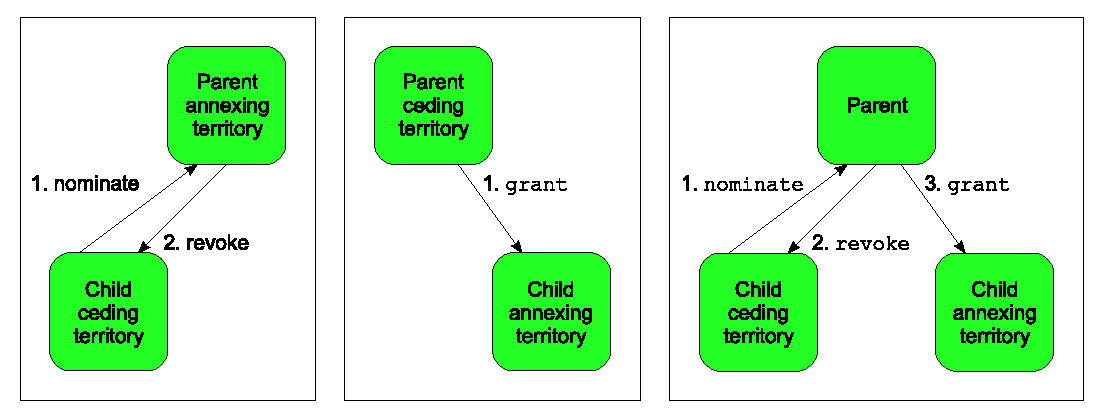
\includegraphics[width=100mm]{figures/grant-topdown}
\caption{Territory migrations are always driven by the parent in the namespace tree, which can annex a neighboring territory, cede territory to another envoy, or coordinates the transfer of a territory from one neighbor to another. For a child to initiate a transfer, it must send a \texttt{nominate} request to the parent, which then carries out the transfer.}
\label{fig:grant-topdown}
\end{figure}

\subsubsection{Transferring state}

When an envoy is granted a new territory, the first thing that it needs is a description of the boundaries. A territory is just a branch of the global namespace hierarchy, so it can be uniquly identified by its root pathname. In addition to that, the parent envoy sends a list of exits from the territory. An exit is a link to an already-established territory that branches off from the one being granted. Since the boundary description may include any number of exits, multiple messages may be required to transmit the full set.

The new owner also receives a full set of active file handles for the new territory. With the 9p protocol, a file handle may identify a opened or unopened files, file or directories used for \texttt{walk} or \texttt{stat} calls, or directories in the process of being read. To facilitate territory changes and transparent crash recovery, the envoy must be able to recreate any state needed to continue a directory read from the number of bytes returned so far in the sequence of reads. Transfers are relatively rare, and transfers that interrupt \texttt{readdir} sequences are even less common, so the prototype simply starts from the beginning and throws away enough data to find the appropriate place in the directory when the need arises.

Every element of state transferred to the new owner, including the boundaries and the file handles, has a counterpart maintained by a partner envoy that must be notified of the changes. The root name comes from the parent, which already knows about the transfer (since it initiated it), but the boundary exits and file handles require that notifications be sent to their respective envoys. The previous owner is a special case, and since it is also identified in the grant sequence, the new owner can safely assume that the old has completely adjusted to the new order of things and not explicitly notify it of each file handle and shared border the two have in common. Some may also be local to the new owner; good territory assignments regularly bring the territory to the main user, so this is a good result for file handles. For all others, the grant recipient sends a notification immediately, grouping multiple entries going to the same remote envoy when appropriate.

The other side of the process is having a territory ownership revoked. As with all such operations, the process is coordinated by the parent. Viewed strictly as a bilateral arrangement, every revoke appears to the child as a merger of a subtree into its parent, though for convenience it is given a hint about where the territory is going to end up.

A revoke operation works much like a grant operation in reverse: the envoy receives a revoke message identifying the root of the territory, and it responds by sending back the current borders and active file handles. It updates its own state for local file handles that become remote, but otherwise leaves updates to the new owner as described above. This is important for synchronizing the transfer with client requests, as detailed below.

Together with \texttt{nominate} messages, grant and revoke transactions give full flexibility for arranging territories. An envoy may cede part of its territory by granting it to a remote envoy and establishing a parent/child relationship with it. An owner may likewise cede its territory to the parent or to a third envoy by issuing a nominate request. Compound requests that carve up territories in more detail are not directly supported, though some could be simulated through sequences of transactions. In general, complicated control decisions made by a central player are avoided in preference to localized choices. The owner of a territory is the only envoy that knows the recent history of requests, and is thus best suited to make realignment decisions.

\subsubsection{Inflight operations}

Top-down coordination of synchronized transactions helps prevent deadlock, but other synchronization issues still exist in territory boundary changes. File operations may be at any stage of completion when the transfer begins, and all must complete successfully without interrupting the client.

The prototype is designed to favor simplicity over other virtues in complex transactions, and this is no exception. Each participant in a migration waits for all inflight transactions directly involving the territory in question to complete before locking it and queuing up any further incoming requests. When the transfer is complete, the lock is released and the queue examined. Significantly, a revoke transaction always completes after a grant (when the two are paired) and after all other envoys involved have been notified of the change. For some requests this will result in nothing more than a pause, while for others the immediate consequence is a failed result. The envoy may no longer recognize a file handle that has been transferred, and can do no more than send the request back to its originator to try again. Note that forwarding it as a special case is an option, but a dangerous one. The message could still end up at the wrong place due to bad timing (and a second transfer of the target), it would involve just as many network round trips (originator to old owner to new owner vs.\ originator to old owner followed by originator to new owner), and the new owner would reject the request anyway as coming from the wrong owner (recall that remote file handles are associated with the client's envoy).

\prettyref{fig:migrate-sync} illustrates a request that conflicts with a territory transfer. A request coming from a client's envoy that reaches its target before the territory is locked is allowed to run to completion. If it arrives after the lock, then it is suspended (this is true if the territory owner is the same as the client's envoy, or if it is remote). The revoke transaction only completes after the corresponding grant has completed and the client's envoy has been notified of the update, so when the old owner bounces the request back, the client's envoy knows the new forwarding address and can immediately retry the request with the new owner. If a request comes after a particular file handle has been updated but before the grant has completed, the new owner simply holds the request until the transfer transaction is complete, at which point it can safely start processing requests, even before the revoke operation has been finalized.

\begin{figure}[tp]
\centering
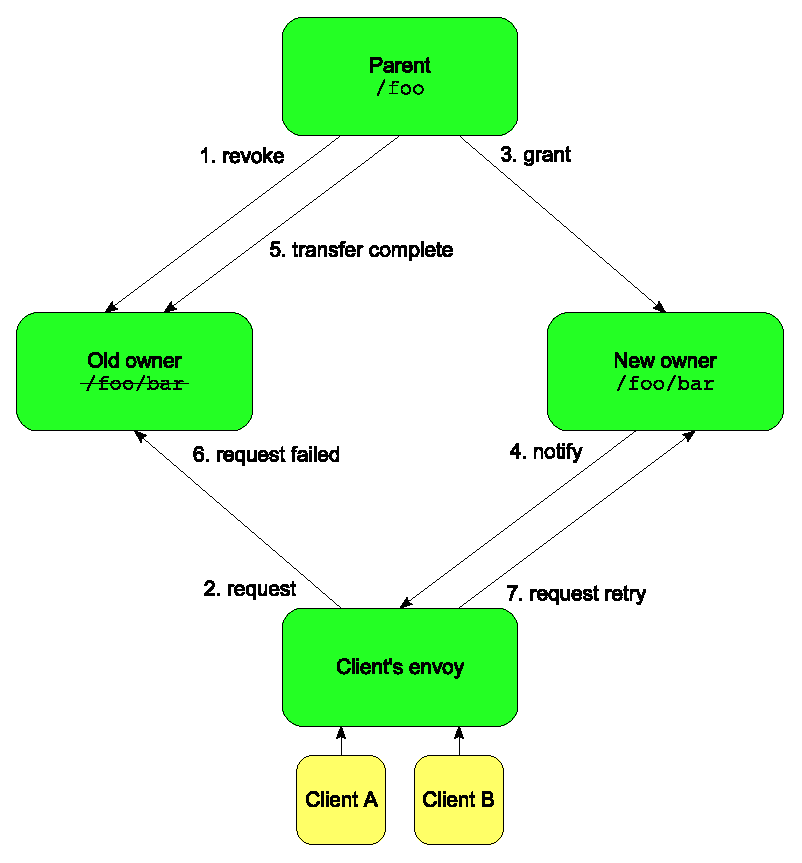
\includegraphics[width=100mm]{figures/migrate-sync}
\caption{The sequence of events when a client file request conflicts with a territory transfer.}
\label{fig:migrate-sync}
\end{figure}

\section{Caching}

\section{Summary}
\chapter{Evaluation}\label{cha:evaluation}

Envoy is designed based on assumptions about a platform that does not yet exist. This limits how the system can be evaluated in two ways. The first is scalability. While common bottlenecks can be avoided and the architecture examined for potential scalability limitations, a system without a large-scale implementation can never be fully tested for issues that only appear at large scales. The best that can be achieved is to identify the most likely sources of problems and extrapolate the results of testing on a smaller scale. The architecture can also be evaluated against assumptions about the workloads it is intended to support, which leads to the second limitation: workloads cannot be accurately forecast. Predicting and simulating client access patterns is a difficult problem even for existing environments \cite{ganger95}, and the problem is amplified for service clusters. As a general purpose platform, service clusters are intended to support a wide range of existing workloads and to enable a flourishing ecosystem of computation services that create entirely new workloads. The design and the evaluation must necessarily rely on assumptions about how the system will be used, and those assumptions limit the applicability of the results.

In this chapter I evaluate the Envoy prototype with three principal goals: to measure the impact of specific design choices, including the basic distributed organisation and cache layout, to assess the scalability of the system, and to evaluate Envoy's ability to support the types of workloads expected in service clusters.

\section{Methodology}

The absence of a realistically sized service cluster limits the scope of system-level testing and the usefulness of many application-level results. The performance side-effects of interacting components and the access patterns of different clients are particularly difficult to predict. The performance characteristics of the storage layer depend on design elements and implementation choices beyond the scope of this dissertation. These factors combined with the poor public availability of many comparable systems limit direct comparisons to previous work.

Building and evaluating a prototype of the Envoy file system is not a futile exercise, however. The artefact may reveal little about real-world usage and behaviour, but measuring it can still do much to justify or condemn the design. The remainder of this section outlines assumptions about service clusters that influence the design, and how measurements of the prototype can quantify the efficacy of the design subject to those assumptions.

\subsection{Overlapping data access}

Cache systems are all built around the premise that a client request for data is a good indicator that it will be accessed again soon. Storing the most recently accessed data in faster storage allows many requests to be absorbed without consulting the primary repository. Coincidental traffic may be due to external factors, e.g., multiple people influenced by the same popular culture event request the same article from Wikipedia, or to structural factors, e.g., multiple clients booting the same Linux distribution access many of the same files, as well as to random overlap. Repetition is also standard within the context of a single client, where a small set of applications, configuration files, and data files tend to be used more than the rest. In addition, file system and application semantics create locality in access patterns by grouping files into directories that must be queried multiple times to complete common tasks.

Envoy assumes that skewed access distributions will continue to be a feature of future workloads just as it is of current workloads. Furthermore, it uses template images to encourage implicit sharing between clients. Caching is managed at the machine level, with a single in-memory and on-disk pool for all of the clients hosted on that node. Client behaviour cannot always be predicted, but the tradeoffs of this cache model can be evaluated. \secref{sec:architectural-costs} compares the performance of the in-memory and on-disk caches with access to the uncached storage layer, and also discusses the cost of a single machine-level cache over per-client caching. These measurements compare the performance gains and losses that can be directly attributed to the cache model, and \secref{sec:quantifying-sharing} applies the results to the assumed model of implicit sharing between clients using the same template image.

\subsection{Independent clients}

* independent boot images, and dynamic transfers to keep them independent as much as possible
* scalability

\subsection{Sharing}

* dynamic transfers--sharing should only happen when there is actual sharing
* keep access to a single cache even when sharing--compare dist lock (flushing to storage layer when token is transferred) to the extra network hop using a single cache

\subsection{scalability}

* assumption is that it is scalable?  more of an argument than an evaluation: envoys don't interact unless they are sharing something (including a border), storage layer mostly consulted for writes(?), but number of spindles grows with the size of the cluster anyway
* what is actually tested here to prove this?




What is this evaluation trying to prove?  What is it not trying to prove?

1. Feasibility: why this isn't a crackpot design
2. Scalability: why this should work for large systems
3. Suitability: why this design matches the requirements

\subsection{Architecture}
* validate the basic goals envoy tries to achieve
* overheads of data paths, justify cache design and territory system
* aggregate caching benefits and costs

\subsection{Dynamic behaviour}
* does the dynamic algorithm work?
* does it serve isolation clients
* does it serve shared clients
* what are the weaknesses

\subsection{Test machines}

\subsection{Benchmarks}

\subsubsection{Linux source tree}
untar -- write test

tar > /dev/null -- read test

rsync -- 2nd read test

\subsubsection{Bonnie}

\section{Performance}

If the goal is to get stuff as local as possible, quantify the benefits of achieving that. Measure the overheads of data paths and cache decisions.

\subsection{Architectural costs}\label{sec:architectural-costs}

userspace NFS

userspace 9p

envoy local dom0

envoy local domU

envoy remote dom0

envoy remote domU

cache: cold vs warm vs hot

\subsection{Fancy features}
\subsubsection{Forks}

cheap and fast---these always happen from a read-only snapshot

\subsubsection{Snapshots}

single territory, many territories

untar the kernel while a bunch of snapshots happen and measure the impact

\subsubsection{Territory migration}

\section{Scalability}
\subsection{Independence of private images}
\subsection{Degradation of a single host with many clients}
Shared image, and also private images on one machine

\subsection{Quantifying sharing}\label{sec:quantifying-sharing}

SUSE10 upgrade, install services

compare image overlap

boot two related images (one cold and other warm) and compare with the same test for identical images

show sharing: boot one VM from cold cache, boot another based on same template

\section{Dynamic behaviour}

Test dynamic territory management, less about performance than behaviour

\subsection{Example scenarios}

shared image with (independent) home directories

2 log files in one directory

producer-consumer

\subsection{Sharing application}
distcc or something else that shares in a complex but predictable fashion

\subsection{Synthetic workloads}

probabilistic traffic driven to overlapping areas

\section{Summary}

\chapter{Conclusion}\label{cha:conclusion}

This dissertation concludes with a discussion of opportunities for future research and a summary of the work presented here.

\section{Future Work}

Storage clusters are only partially specified in this work, and much additional research is necessary to make them a reality. Even the storage component that is the focus of this dissertation is only partially specified. Also, some parts of the existing design point to areas for future work. A few of these areas are addressed in this section.

\subsection{Storage layer}

The prototype implementation of Envoy relies on a simplistic storage layer that is statically allocated and managed. Much of the work discussed in \secref{sec:storage-layer-systems} could be applied to create a robust and performant storage service. 

\subsection{Envoy}

\subsection{Read-only leases}
\subsection{Custom protocol}
Cache at client for unshared objects, at envoy for shared
\subsection{Storage-informed load balancing}
\subsection{Recovery}

\section{Summary}


% bibliography

\clearpage
\singlespace
\renewcommand{\bibname}{References}
\addcontentsline{toc}{chapter}{\bibname}

% hardcode the headers so they are not uppercase
\makeatletter
  \if@twoside
    \lhead[\fancyplain{}{\sffamily\small\textsl{\bibname}}]{}
    \rhead[]{\fancyplain{}{\sffamily\small\textsl{\bibname}}}
  \else
    \lhead[]{\fancyplain{}{\sffamily\small\textsl{\bibname}}}
  \fi
\makeatother

\bibliographystyle{plain}
\bibliography{references}

\end{document}
